%%%%%%%%%%%%%%%%%%%%%%%%%
% Dokumentinformationen %
%%%%%%%%%%%%%%%%%%%%%%%%%
\newcommand{\titleinfo}{PMSwEng Zusammenfassung}
\newcommand{\authorinfo}{Gian Claudio Koeppel}
\newcommand{\versioninfo}{$Revision: 1 $ - powered by \LaTeX}

%%%%%%%%%%%%%%%%%%%%%%%%%%%%%%%%%%%%%%%%%%%%%
% Standard projektübergreifender Header für
% - Makros 
% - Farben
% - Mathematische Operatoren 
%
% DORT NUR ERGÄNZEN, NICHTS LÖSCHEN
%%%%%%%%%%%%%%%%%%%%%%%%%%%%%%%%%%%%%%%%%%%%%  
%%%%%%%%%%%%%%%%%%%%%%%%%%%%%%%%%%%%%%%
%% Makros & anderer Low-Level bastel %%
%%%%%%%%%%%%%%%%%%%%%%%%%%%%%%%%%%%%%%%
\makeatletter
%% Makros für Titel, Autor und Datum 
%% Dank diesem Makro stehen Titel, Autor und Datum überall im Dokument zur verfügung
%% Date hat zudem den Default-Wert \today
\def\@Title{}
\def\@Author{}
\def\@Date{\today}
\newcommand{\Title}{\@Title}
\newcommand{\Author}{\@Author}
\newcommand{\Date}{\@Date}
\AtBeginDocument{%
  \let\@Title\@title
  \let\@Author\@author
  \let\@Date\@date
}

%% Makros für den Arraystretch (bei uns meist in Tabellen genutzt, welche Formeln enthalten)
% Default Value
\def\@ArrayStretchDefault{1} % Entspricht der Voreinstellung von Latex

% Setzt einen neuen Wert für den arraystretch
\newcommand{\setArrayStretch}[1]{\renewcommand{\arraystretch}{#1}}

% Setzt den arraystretch zurück auf den default wert
\newcommand{\resetArrayStretch}{\renewcommand{\arraystretch}{\@ArrayStretchDefault}}

% Makro zum setzten des Default arraystretch. Kann nur in der Präambel verwendet werden.
\newcommand{\setDefaultArrayStretch}[1]{%
	\AtBeginDocument{%
		\def\@ArrayStretchDefault{#1}
		\renewcommand{\arraystretch}{#1}
	}
}
\makeatother



\usepackage[automark]{scrpage2} % Header und Footer


% Seitenränder
\geometry{left=1.5cm,right=1cm,top=1cm,bottom=1cm,includeheadfoot}
\usepackage[T1]{fontenc}

%%%%%%%%%%%%%%%%%%%%%%%%%%%%%%%%%%%%%%%%%%%%
\usepackage[final]{pdfpages}
% Syntaxhighlighting für Code
\usepackage{listings}
%\usepackage{textcomp}
\definecolor{lbcolor}{rgb}{0.92,0.92,0.92}
\lstset{
backgroundcolor=\color{lbcolor},
tabsize=4,
rulecolor=,
language=c++,
    basicstyle=\scriptsize\ttfamily,
    upquote=true,
    aboveskip={0.5\baselineskip},
    columns=fixed,
    showstringspaces=false,
    extendedchars=true,
    breaklines=true,
    prebreak = \raisebox{0ex}[0ex][0ex]{\ensuremath{\hookleftarrow}},
    frame=single,
    showtabs=false,
    showspaces=false,
    showstringspaces=false,
    identifierstyle=\bfseries\ttfamily,
    keywordstyle=\color[rgb]{0,0,1},
    commentstyle=\color[rgb]{0.133,0.545,0.133},
    stringstyle=\color[rgb]{0.627,0.126,0.941},
}

\lstset{literate=%
{Ö}{{\"O}}1
{Ä}{{\"A}}1
{Ü}{{\"U}}1
{ß}{{\ss}}2
{ü}{{\"u}}1
{ä}{{\"a}}1
{ö}{{\"o}}1
{°}{{$^{\circ}$}}1
{'}{{}}1
}

\lstset{basicstyle=\ttfamily}
%%%%%%%%%%%%%%%%%%%%%%%%%%%%%%%%%%%%%%%%%%%%
% Möglichst keine Ergänzungen hier, sondern in header.tex
\begin{document}

%Uebung 1
\setcounter{section}{1}
\setcounter{subsection}{0}
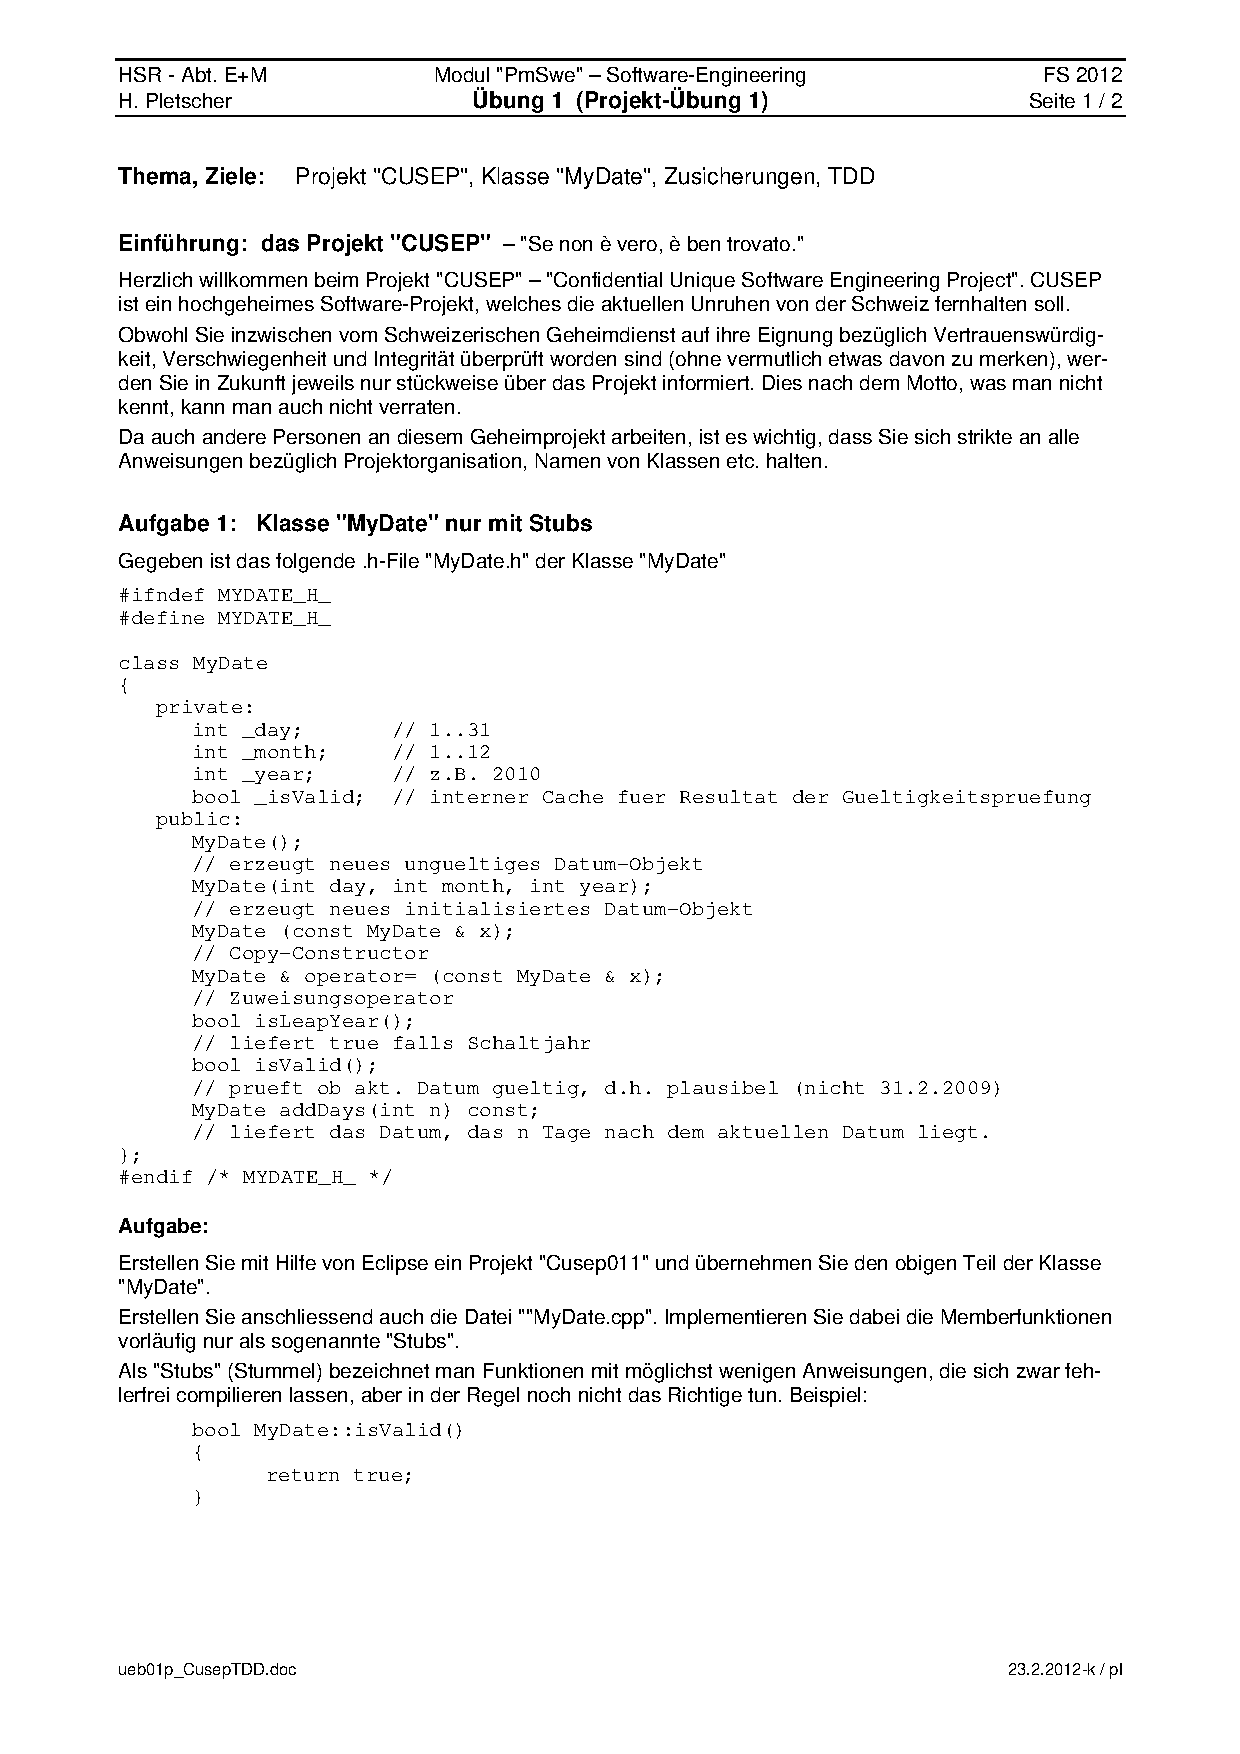
\includepdf[pages=-]{./UebAufgaben/ueb01p_CusepTDD.pdf}
\subsection{Lösung}
\subsubsection{MyDate.h}
\lstinputlisting{./UebLoesungen/LoesUeb01_Cusep1/MyDate.h}
\subsubsection{MyDate.cpp}
\lstinputlisting{./UebLoesungen/LoesUeb01_Cusep1/MyDate.cpp}
\subsubsection{testMyDate.cpp}
\lstinputlisting{./UebLoesungen/LoesUeb01_Cusep1/testMyDate.cpp}

%Uebung 2
\setcounter{section}{2}
\setcounter{subsection}{1}
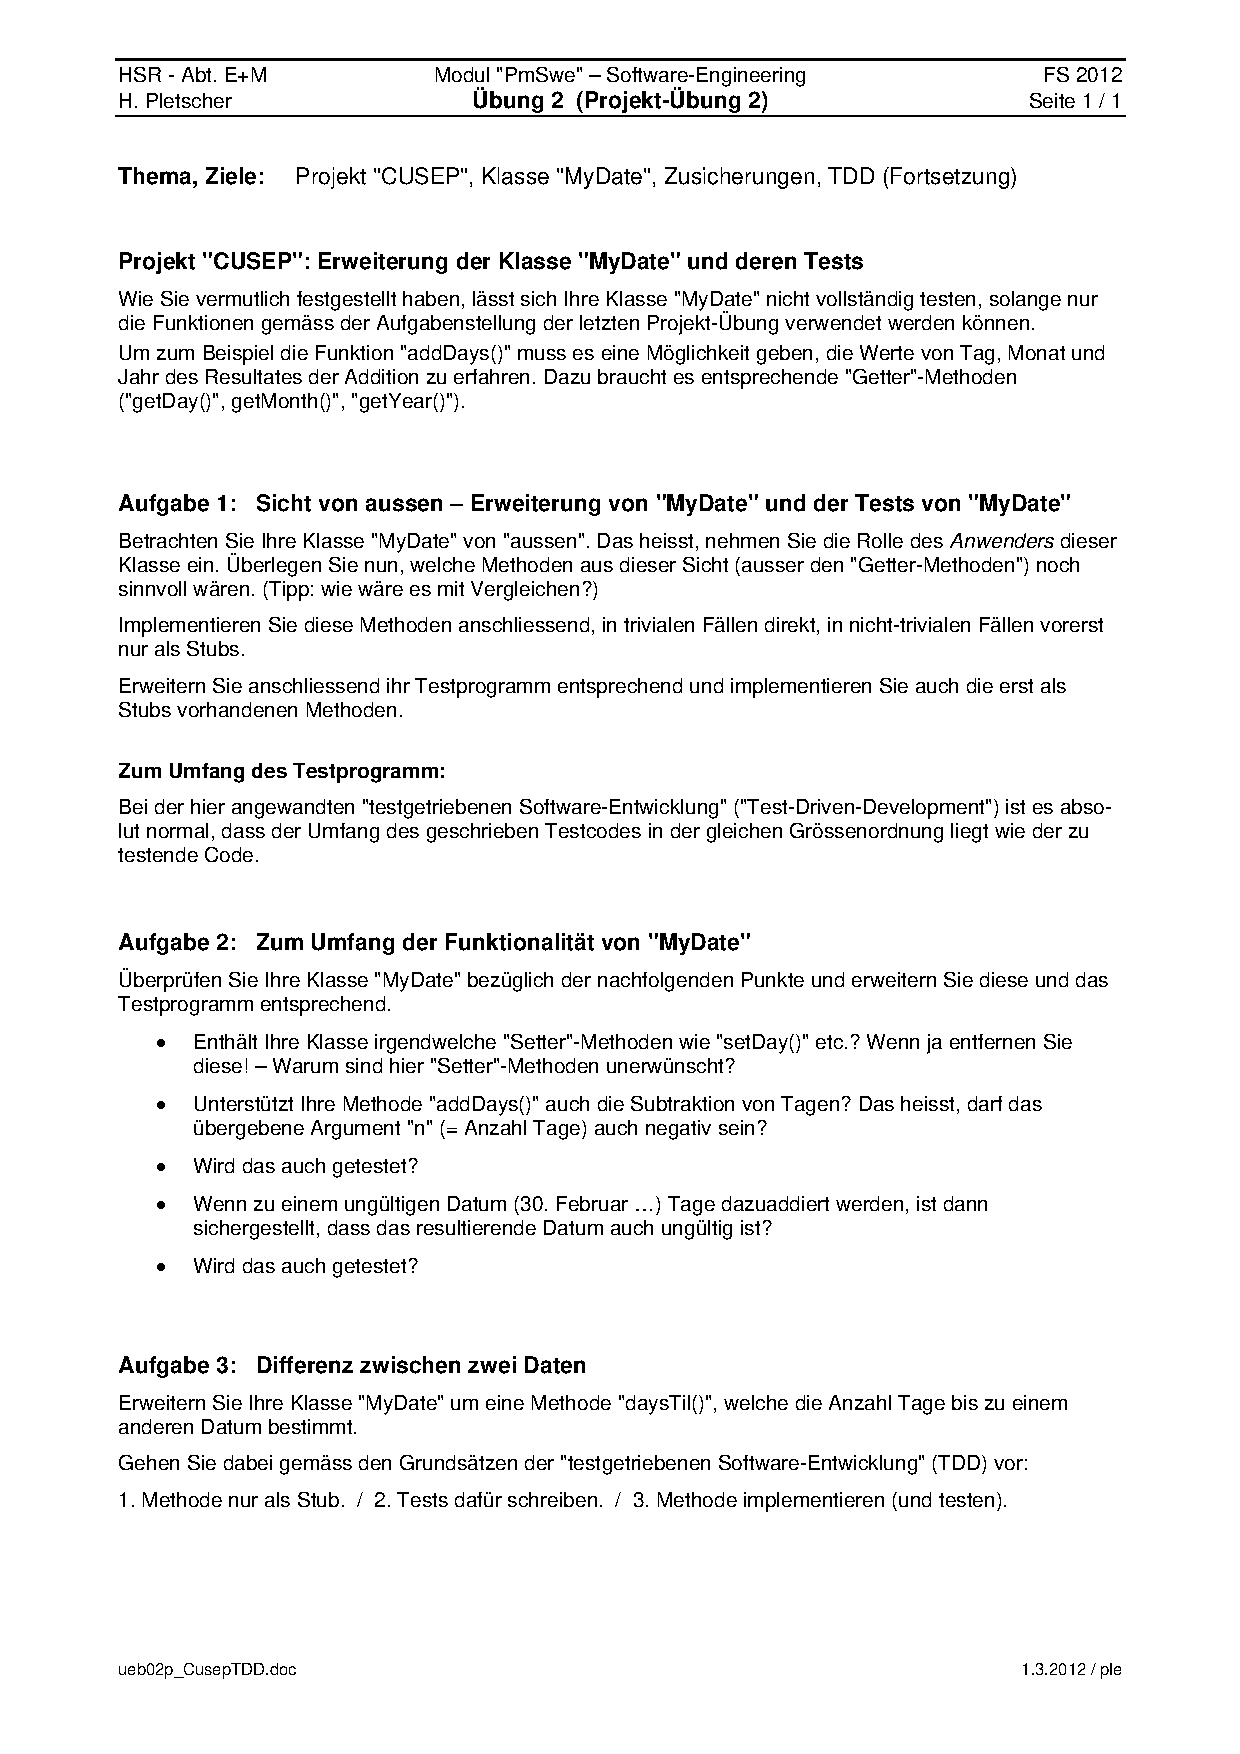
\includepdf[pages=-]{./UebAufgaben/ueb02p_CusepTDD.pdf}
\subsection{Lösung}
\subsubsection{MyDate.h}
\lstinputlisting{./UebLoesungen/LoesUeb02_Cusep2/MyDate.h}
\subsubsection{MyDate.cpp}
\lstinputlisting{./UebLoesungen/LoesUeb02_Cusep2/MyDate.cpp}
\subsubsection{testMyDate.cpp}
\lstinputlisting{./UebLoesungen/LoesUeb02_Cusep2/testMyDate.cpp}

%Uebung 3
\setcounter{section}{3}
\setcounter{subsection}{1}
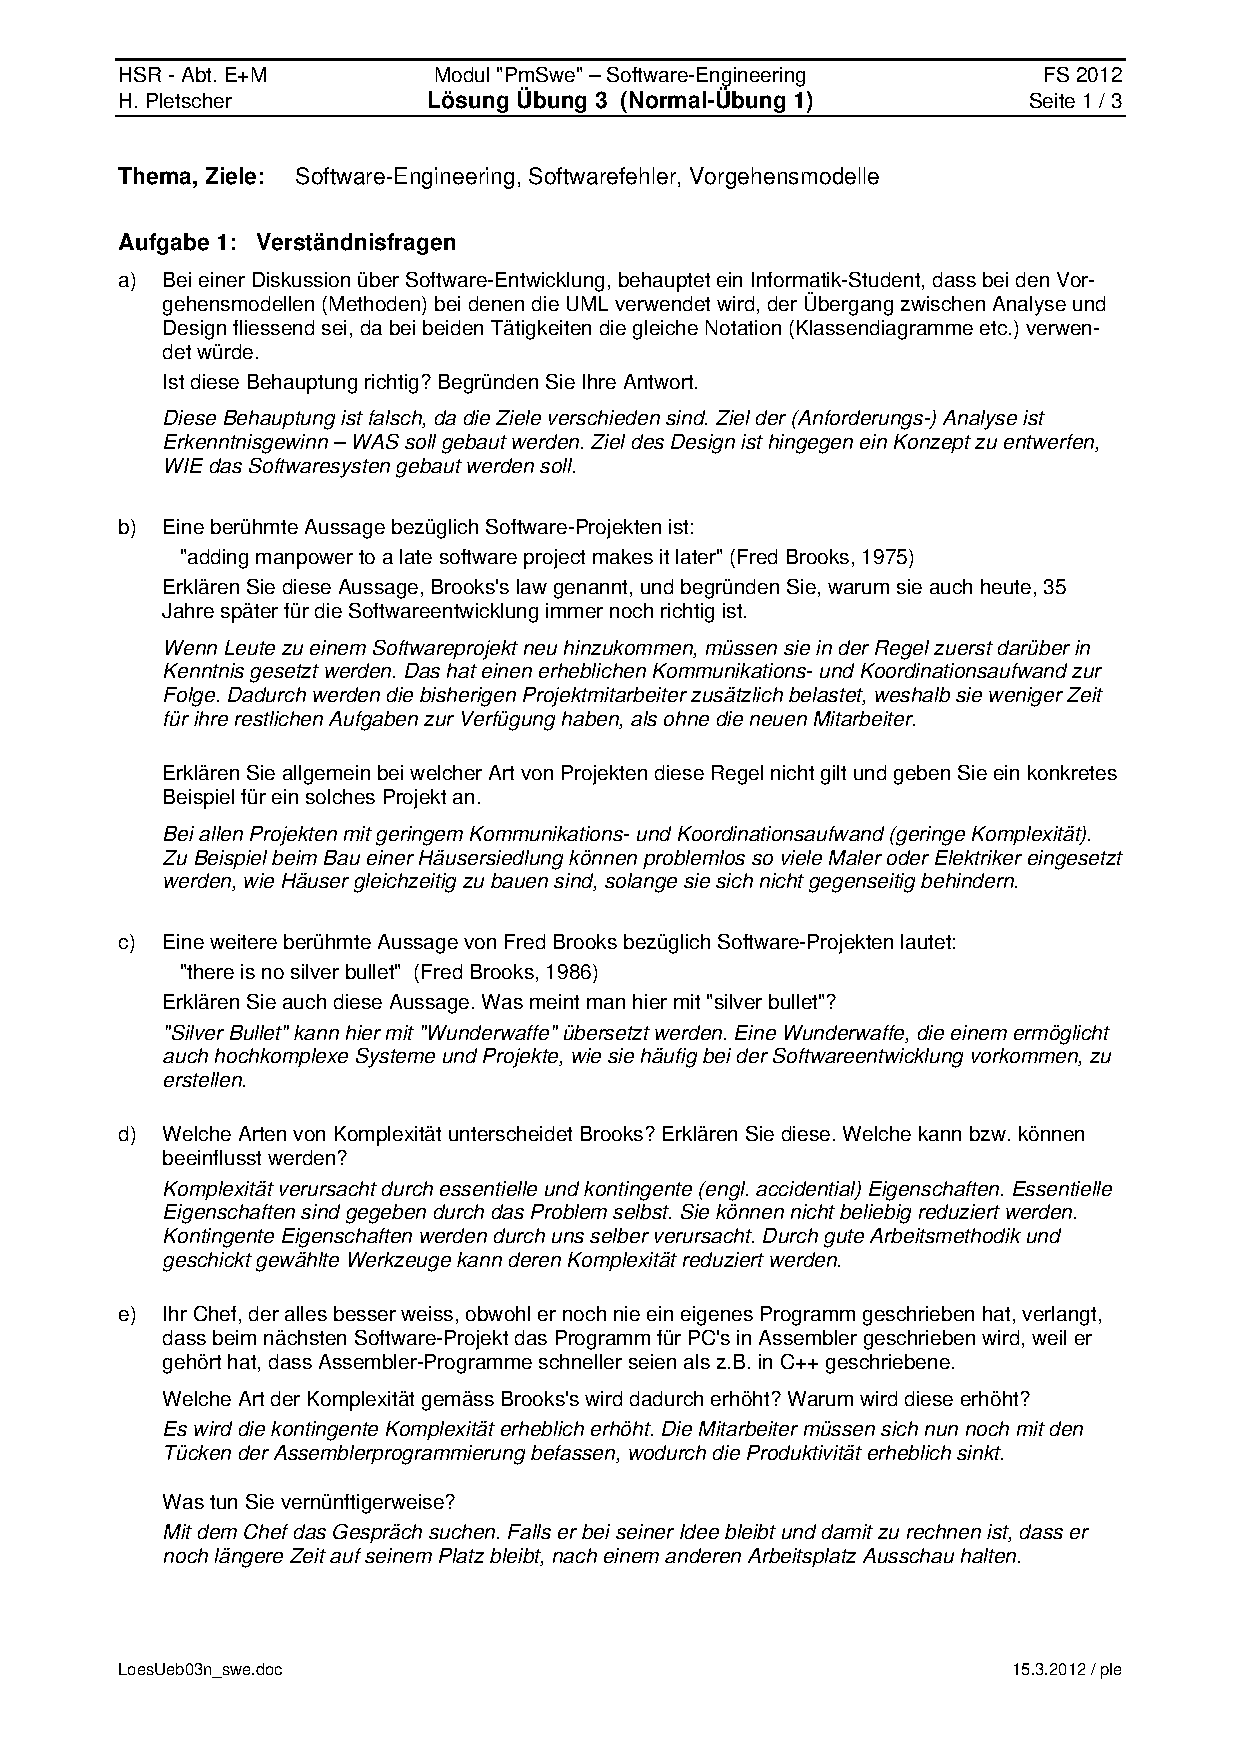
\includepdf[pages=-]{./UebLoesungen/LoesUeb03_swe/LoesUeb03n_swe.pdf}

%Uebung 4
\setcounter{section}{4}
\setcounter{subsection}{1}
\setcounter{subsubsection}{1}
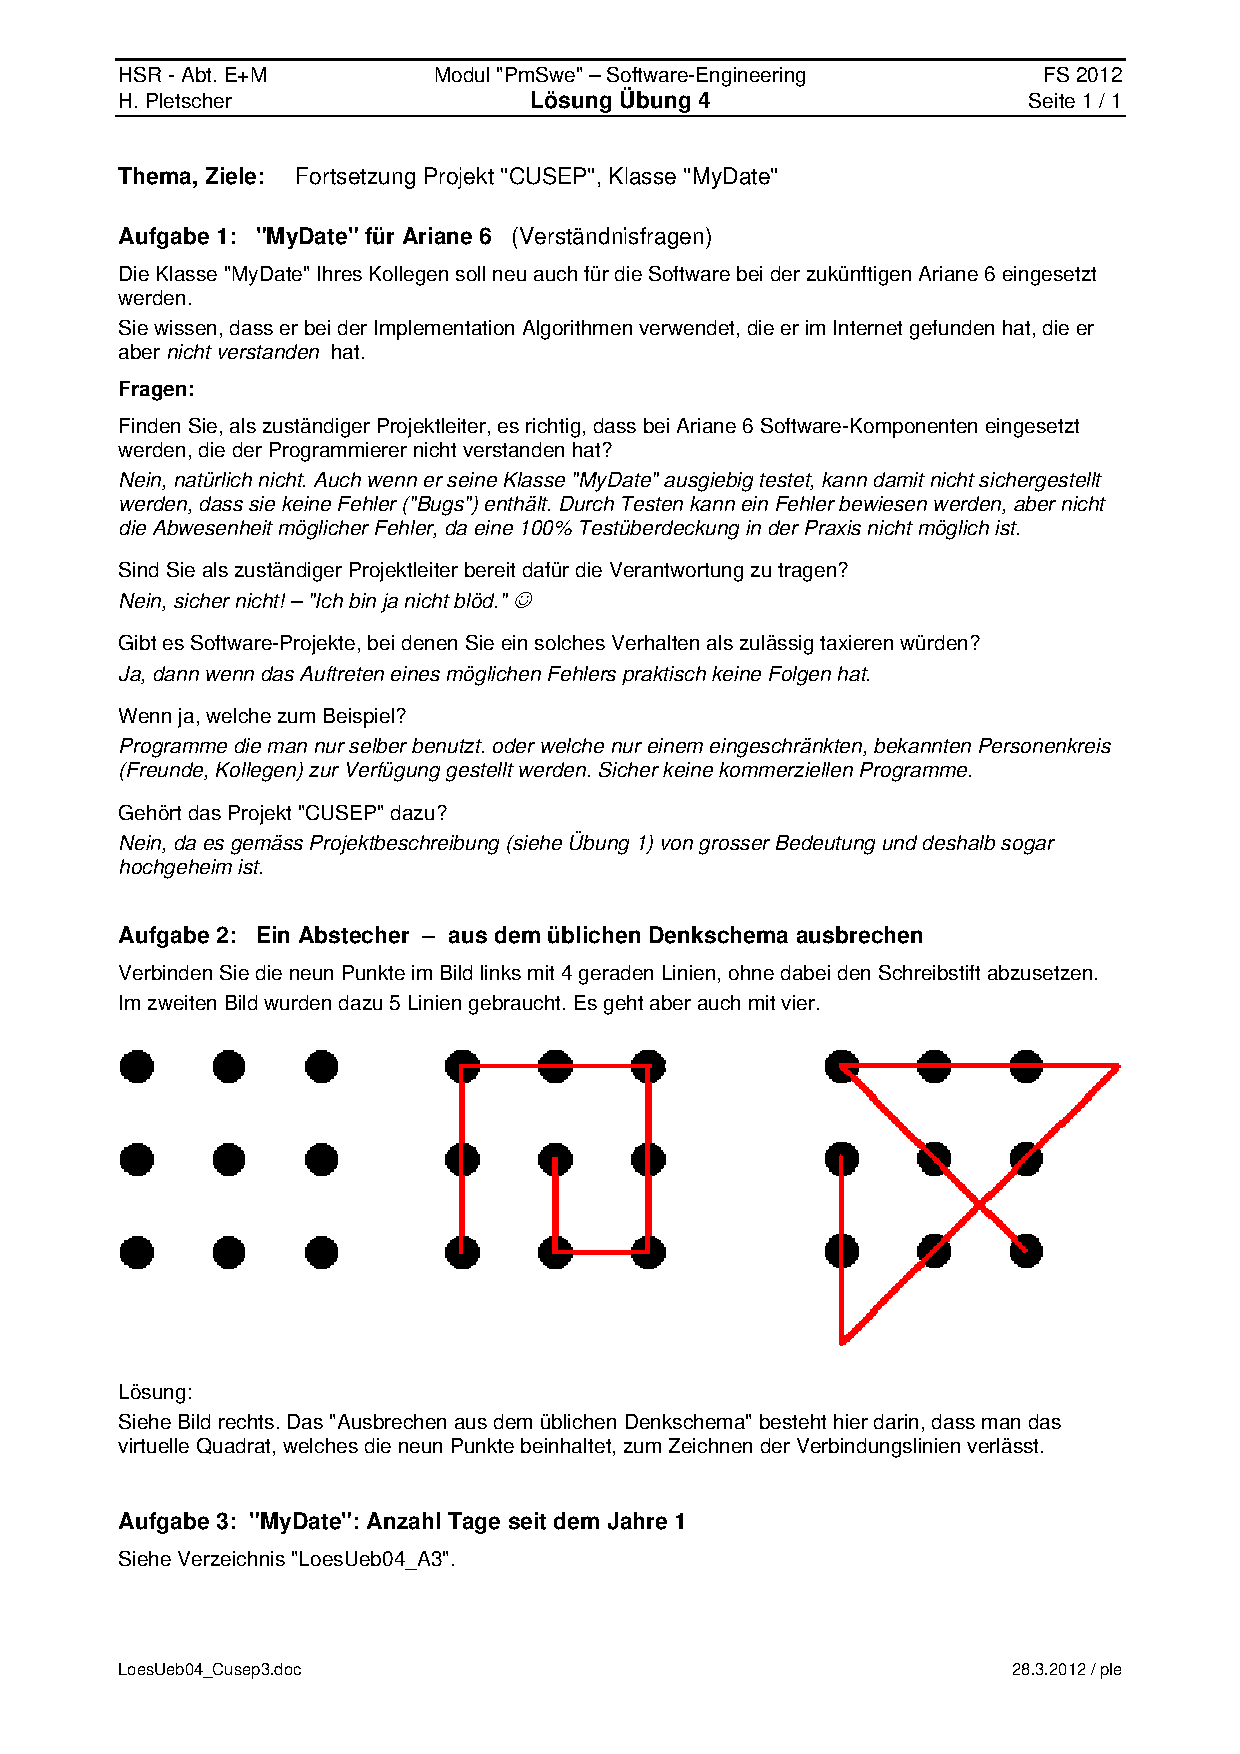
\includepdf[pages=-]{./UebLoesungen/LoesUeb04_Cusep3/LoesUeb04_Cusep3.pdf}
\subsection{Lösung}
\subsubsection{MyDate.h}
\lstinputlisting{./UebLoesungen/LoesUeb04_Cusep3/LoesUeb04_A3_MyDate/MyDate.h}
\subsubsection{MyDate.cpp}
\lstinputlisting{./UebLoesungen/LoesUeb04_Cusep3/LoesUeb04_A3_MyDate/MyDate.cpp}
\subsubsection{testMyDate.cpp}
\lstinputlisting{./UebLoesungen/LoesUeb04_Cusep3/LoesUeb04_A3_MyDate/testMyDate.cpp}

%Uebung 5
\setcounter{section}{5}
\setcounter{subsection}{1}
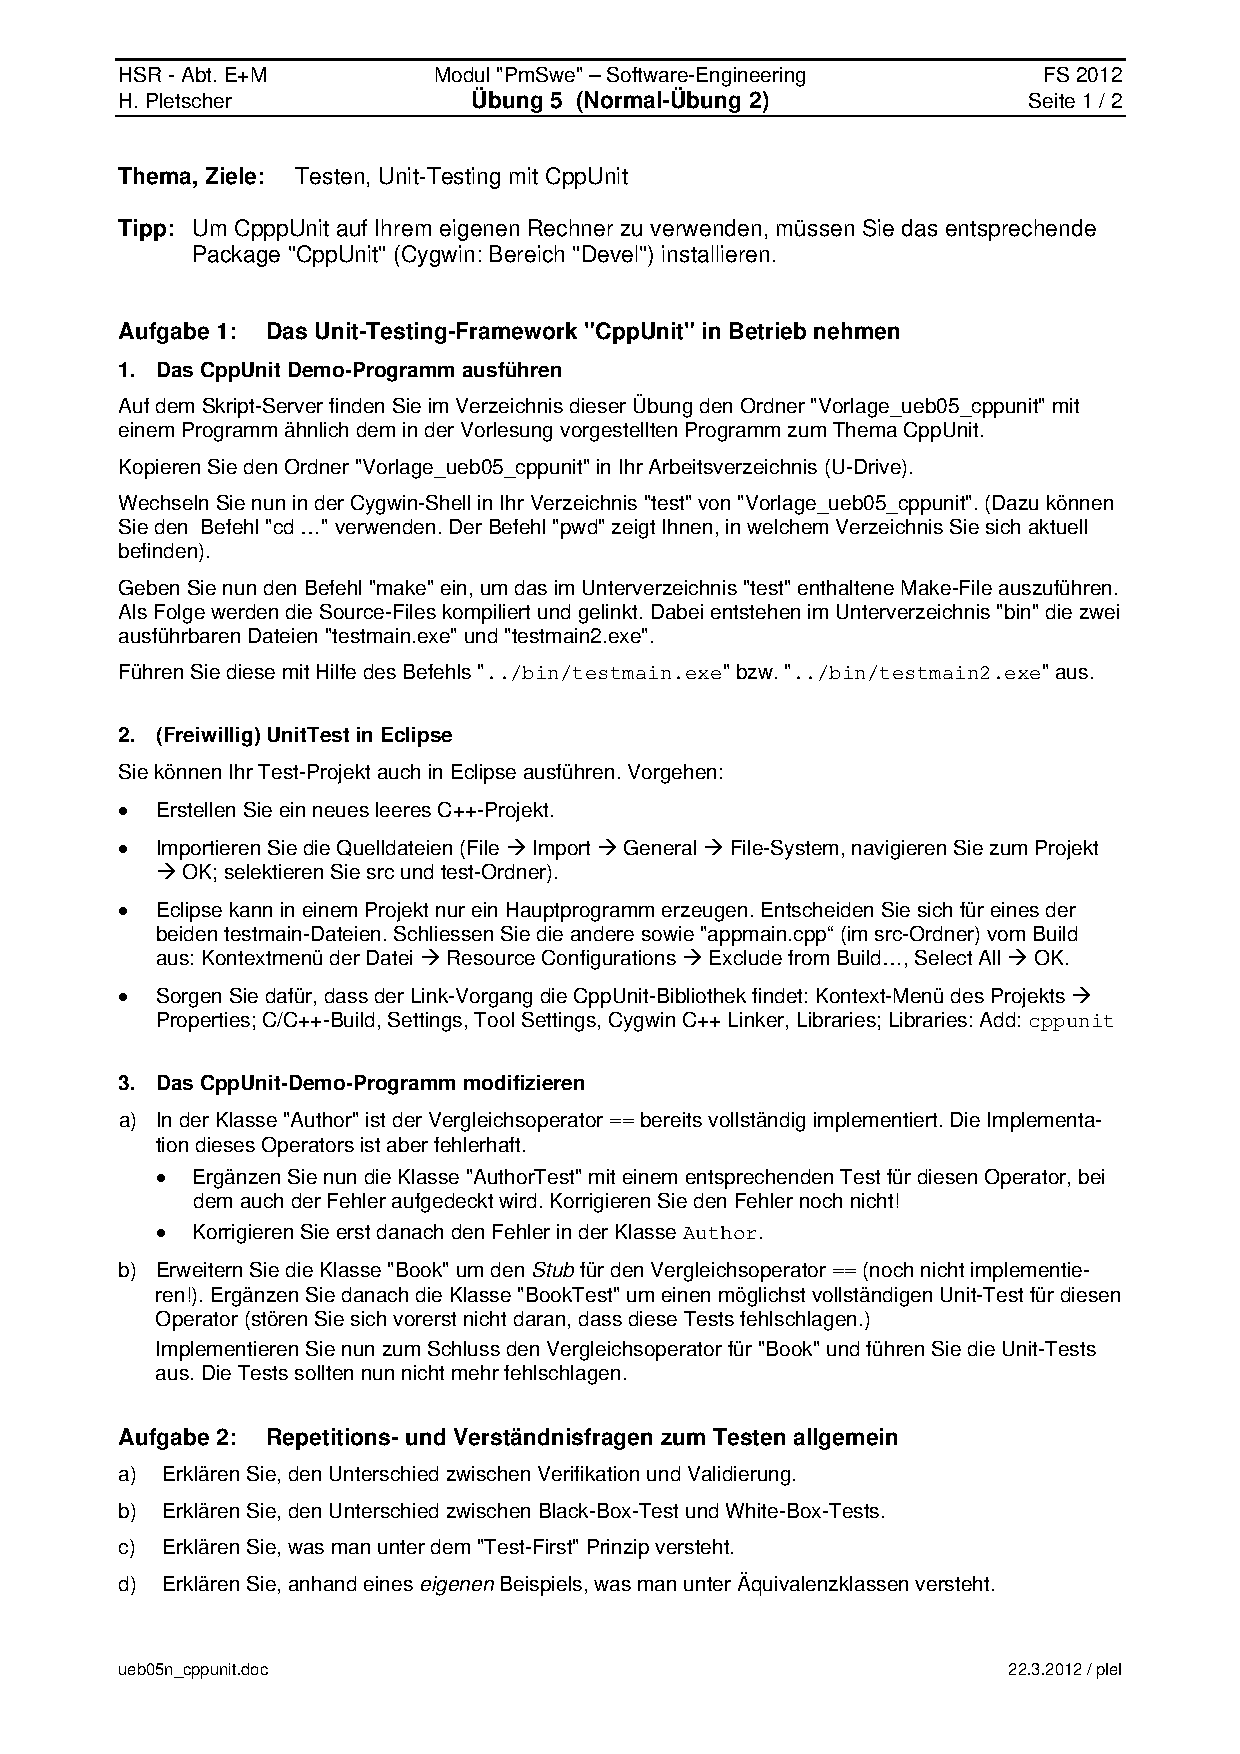
\includepdf[pages=-]{./UebAufgaben/ueb05n_cppunit.pdf}
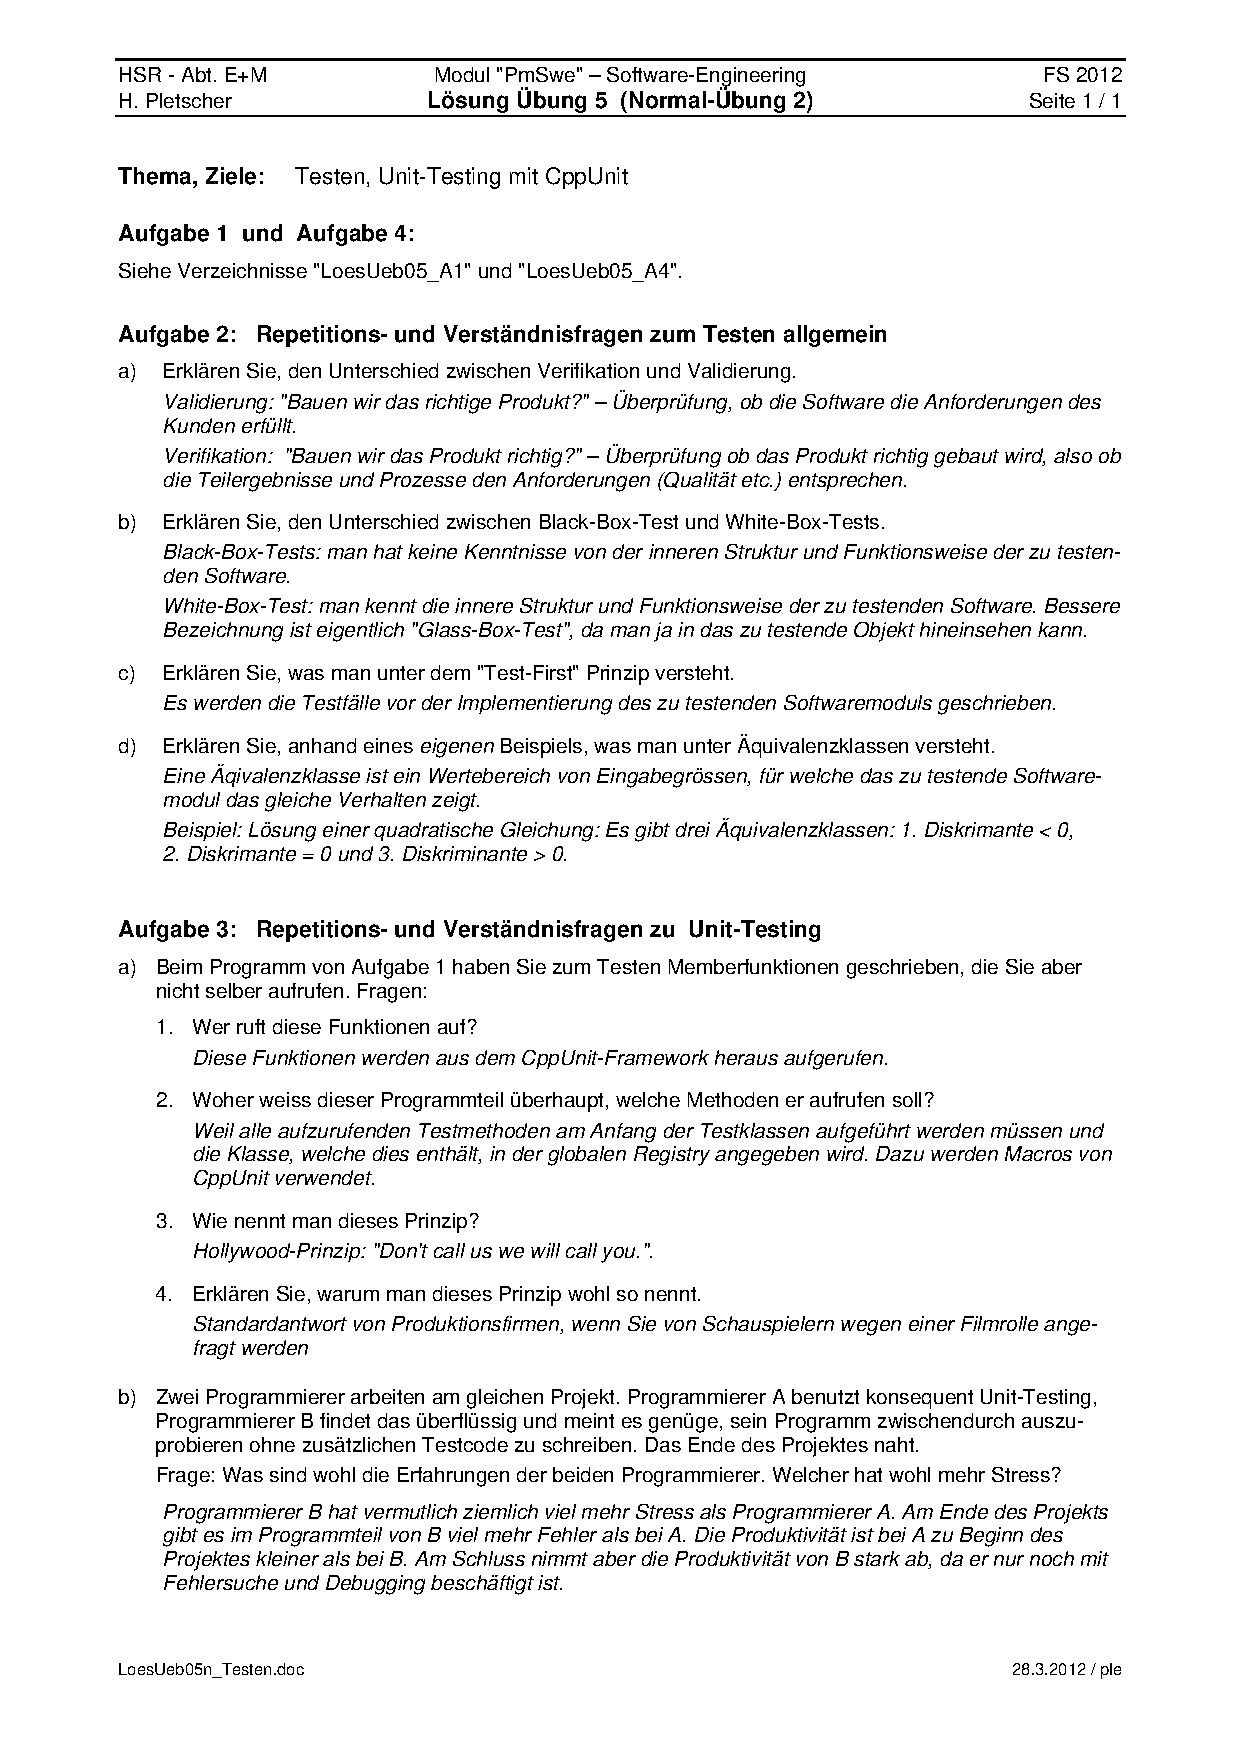
\includepdf[pages=-]{./UebLoesungen/LoesUeb05_testen/LoesUeb05n_Testen.pdf}
\subsection{Lösung Aufgabe 1}
\subsubsection{appmain.cpp}
\lstinputlisting{./UebLoesungen/LoesUeb05_testen/LoesUeb05_A1_cppunit/src/appmain.cpp}
\subsubsection{Author.cpp}
\lstinputlisting{./UebLoesungen/LoesUeb05_testen/LoesUeb05_A1_cppunit/src/Author.cpp}
\subsubsection{Author.h}
\lstinputlisting{./UebLoesungen/LoesUeb05_testen/LoesUeb05_A1_cppunit/src/Author.h}
\subsubsection{Book.cpp}
\lstinputlisting{./UebLoesungen/LoesUeb05_testen/LoesUeb05_A1_cppunit/src/Book.cpp}
\subsubsection{Book.h}
\lstinputlisting{./UebLoesungen/LoesUeb05_testen/LoesUeb05_A1_cppunit/src/Book.h}
\subsubsection{MyTools.cpp}
\lstinputlisting{./UebLoesungen/LoesUeb05_testen/LoesUeb05_A1_cppunit/src/MyTools.cpp}
\subsubsection{MyTools.h}
\lstinputlisting{./UebLoesungen/LoesUeb05_testen/LoesUeb05_A1_cppunit/src/MyTools.h}
\subsubsection{AuthorTest.cpp}
\lstinputlisting{./UebLoesungen/LoesUeb05_testen/LoesUeb05_A1_cppunit/tests/AuthorTest.cpp}
\subsubsection{BookTest.cpp}
\lstinputlisting{./UebLoesungen/LoesUeb05_testen/LoesUeb05_A1_cppunit/tests/BookTest.cpp}
\subsubsection{testmain.cpp}
\lstinputlisting{./UebLoesungen/LoesUeb05_testen/LoesUeb05_A1_cppunit/tests/testmain.cpp}
\subsubsection{testmain2.cpp}
\lstinputlisting{./UebLoesungen/LoesUeb05_testen/LoesUeb05_A1_cppunit/tests/testmain2.cpp}

\subsection{Lösung Aufgabe 4}
\setcounter{subsection}{1}
\subsubsection{MyDate.cpp}
\lstinputlisting{./UebLoesungen/LoesUeb05_testen/LoesUeb05_A4_mydate/src/MyDate.cpp}
\subsubsection{MyDate.h}
\lstinputlisting{./UebLoesungen/LoesUeb05_testen/LoesUeb05_A4_mydate/src/MyDate.h}
\subsubsection{MyDate\_\_.cpp}
\lstinputlisting{./UebLoesungen/LoesUeb05_testen/LoesUeb05_A4_mydate/src/MyDate__.cpp}
\subsubsection{MyDate\_\_.h}
\lstinputlisting{./UebLoesungen/LoesUeb05_testen/LoesUeb05_A4_mydate/src/MyDate__.h}
\subsubsection{MyDateTest.cpp}
\lstinputlisting{./UebLoesungen/LoesUeb05_testen/LoesUeb05_A4_mydate/test/MyDateTest.cpp}
\subsubsection{testmain.cpp}
\lstinputlisting{./UebLoesungen/LoesUeb05_testen/LoesUeb05_A4_mydate/test/testmain.cpp}


%Uebung 6
\setcounter{section}{6}
\setcounter{subsection}{1}
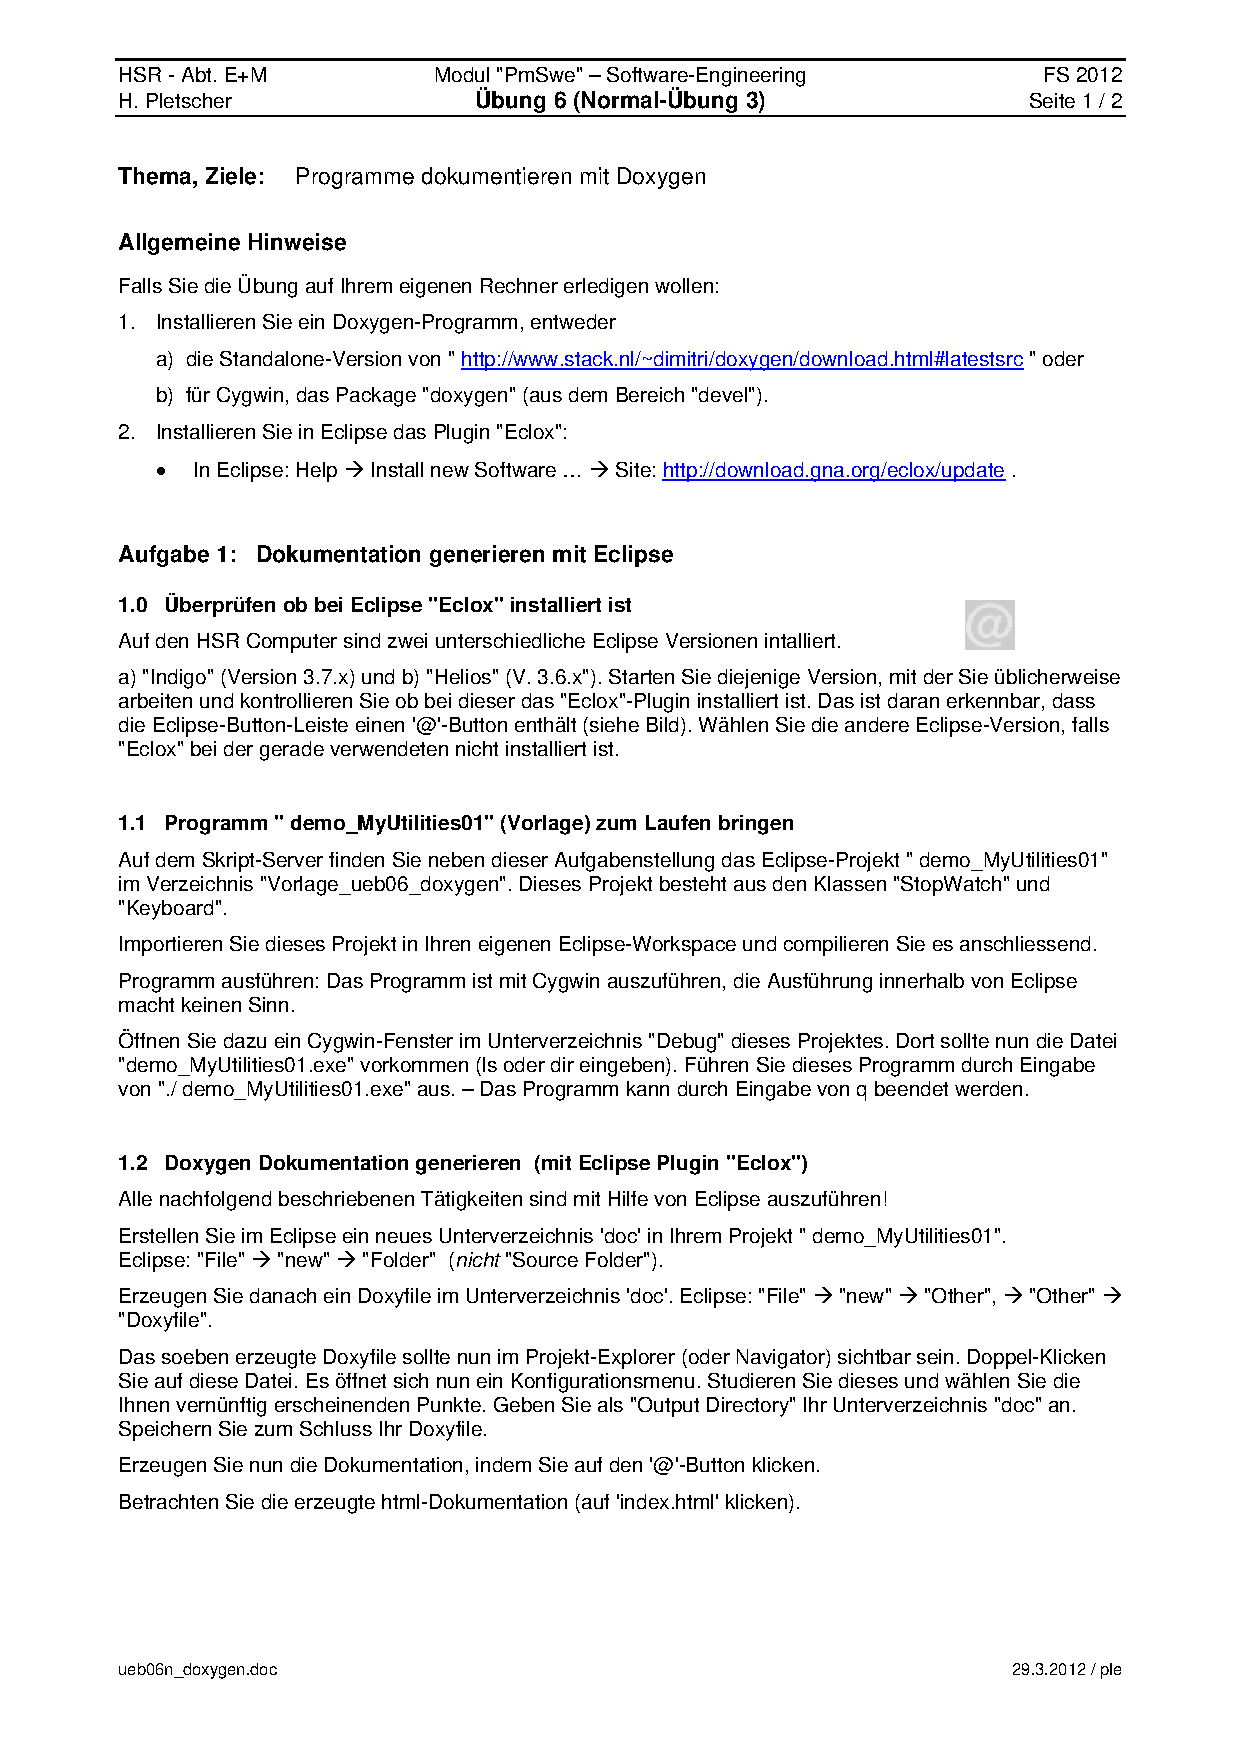
\includepdf[pages=-]{./UebAufgaben/ueb06n_doxygen.pdf}
\subsection{Lösung}
\subsubsection{demo\_MyUtilities01.cpp}
\lstinputlisting{./UebLoesungen/LoesUeb06_doxygen/demo_MyUtilities01.cpp}
\subsubsection{Keyboard.cpp}
\lstinputlisting{./UebLoesungen/LoesUeb06_doxygen/Keyboard.cpp}
\subsubsection{Keyboard.h}
\lstinputlisting{./UebLoesungen/LoesUeb06_doxygen/Keyboard.h}
\subsubsection{mainpage.h}
\lstinputlisting{./UebLoesungen/LoesUeb06_doxygen/mainpage.h}
\subsubsection{StopWatch.cpp}
\lstinputlisting{./UebLoesungen/LoesUeb06_doxygen/StopWatch.cpp}
\subsubsection{StopWatch.h}
\lstinputlisting{./UebLoesungen/LoesUeb06_doxygen/StopWatch.h}

%Uebung 7
\setcounter{section}{7}
\setcounter{subsection}{1}
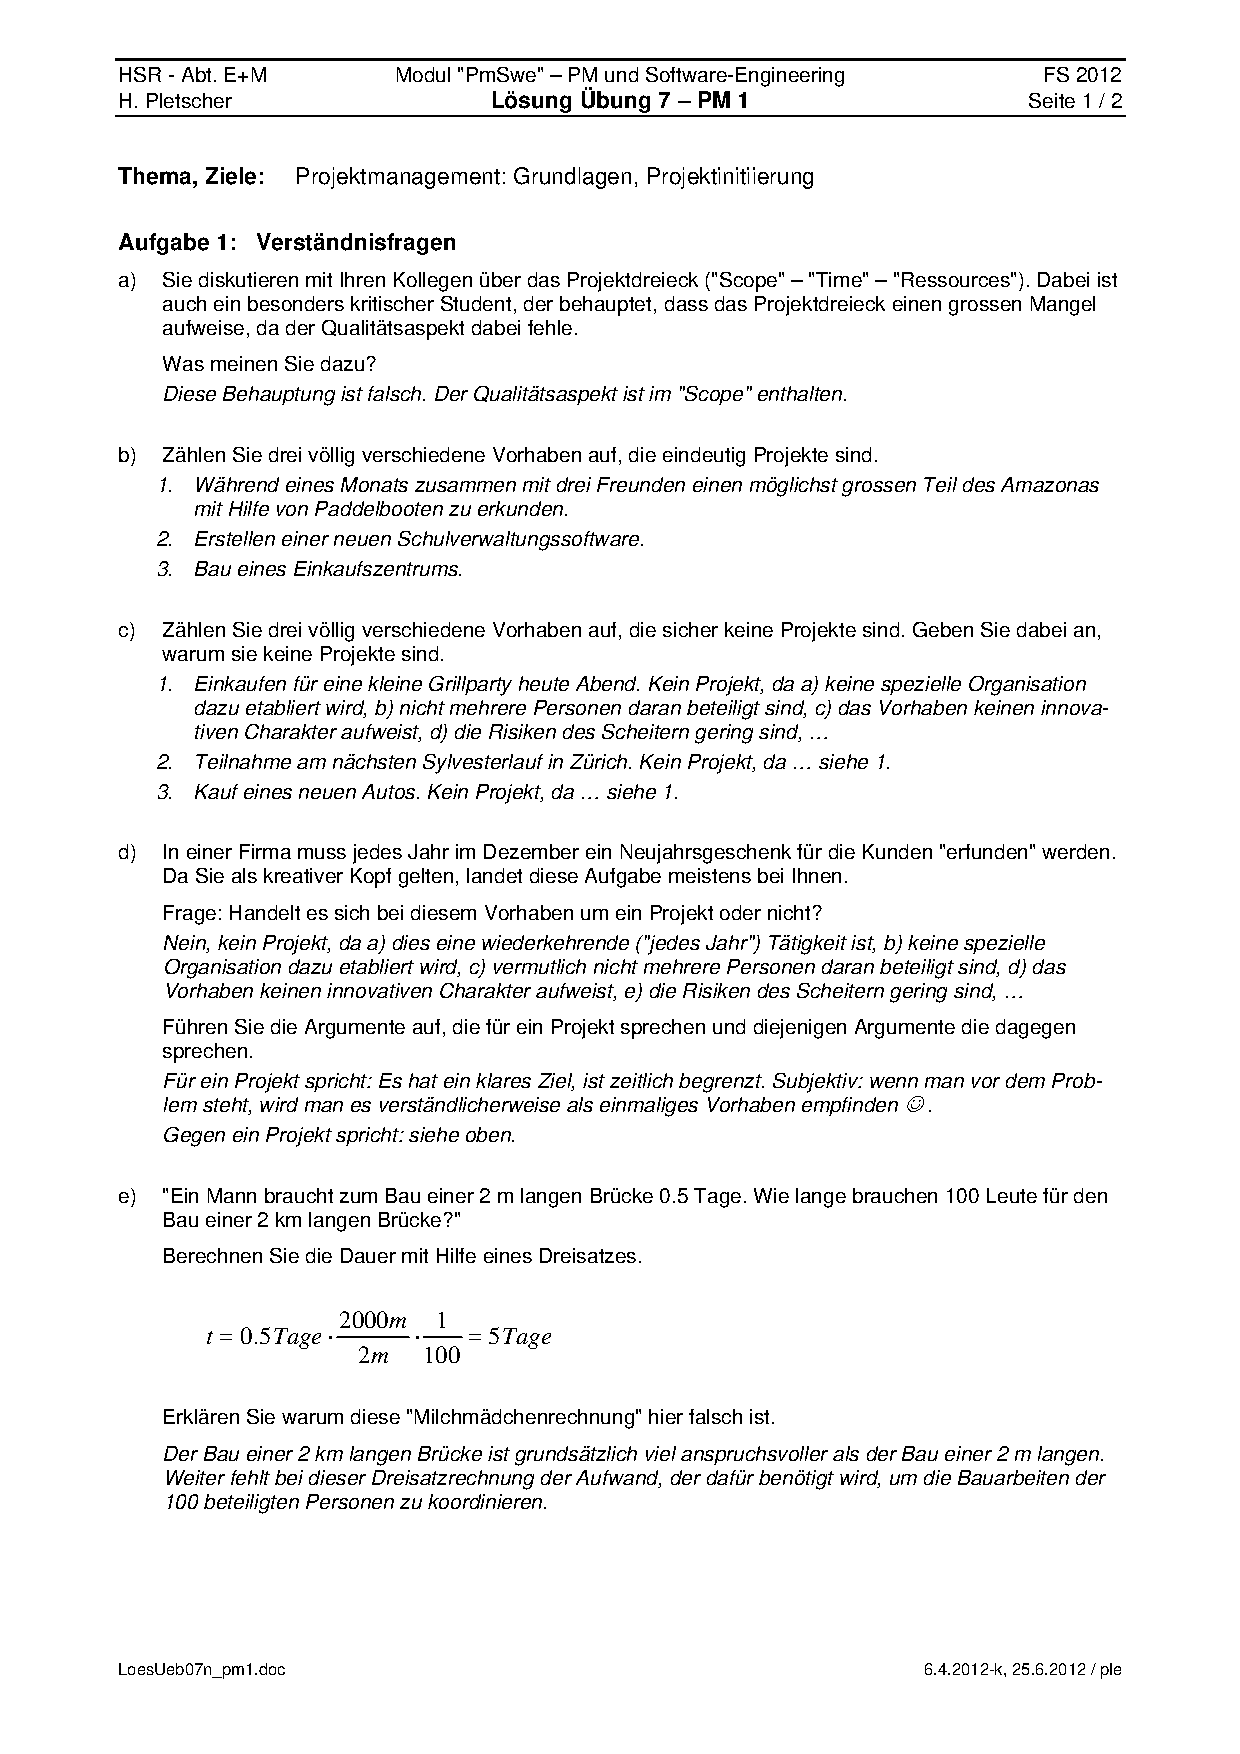
\includepdf[pages=-]{./UebLoesungen/LoesUeb07_pm1/LoesUeb07n_pm1.pdf}

%Uebung 8
\setcounter{section}{8}
\setcounter{subsection}{1}
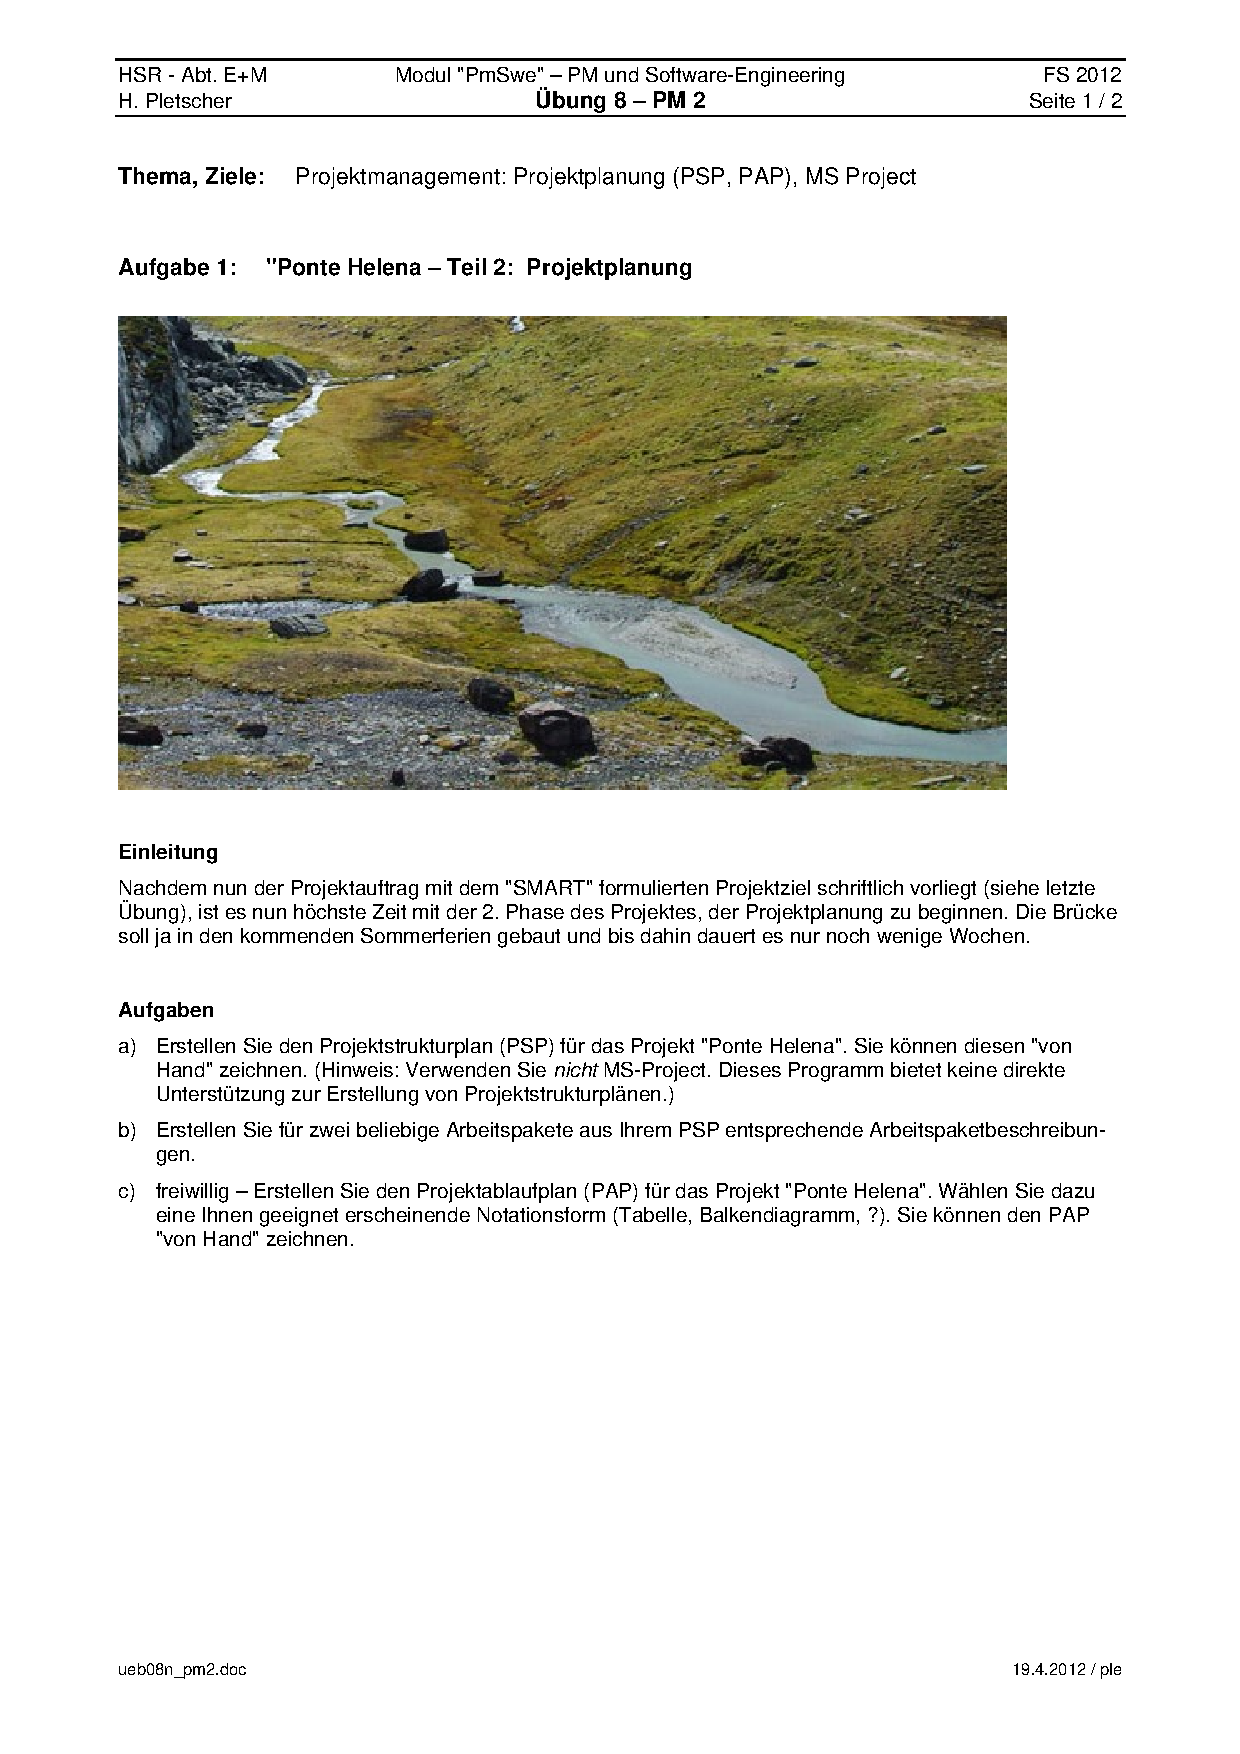
\includepdf[pages=-]{./UebAufgaben/ueb08n_pm2.pdf}
\subsection{Lösung}
\begin{center}
	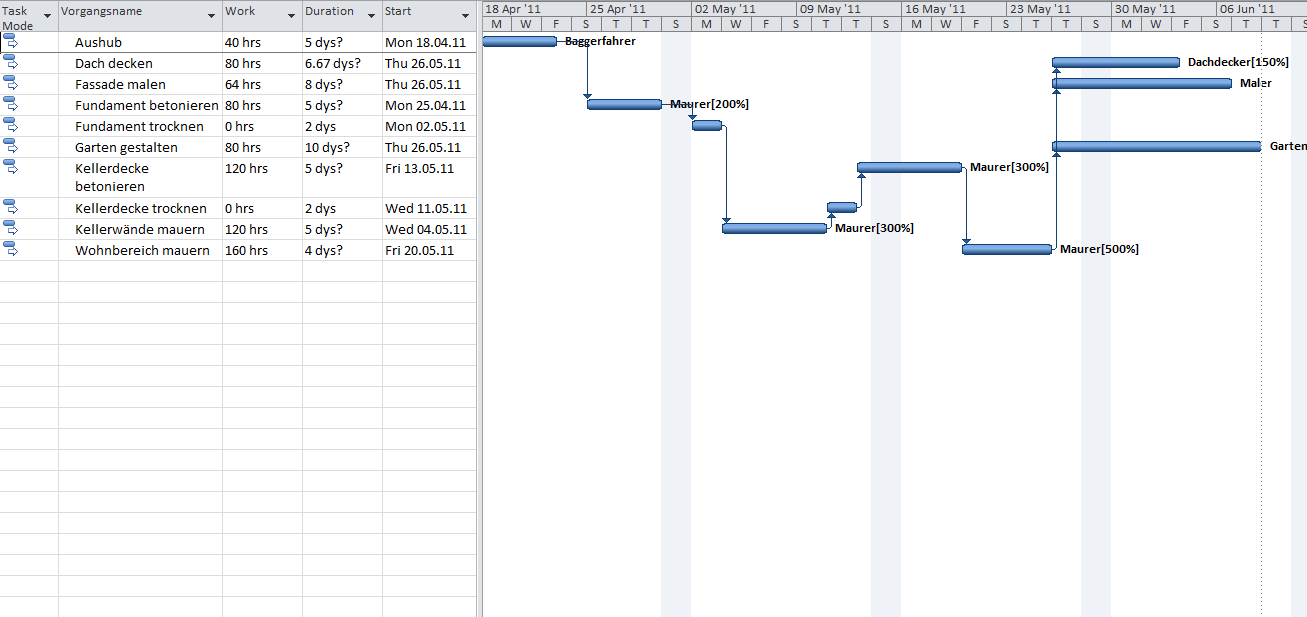
\includegraphics[angle=90,width=0.62\textwidth]{./UebLoesungen/LoesUeb08_pm2/ueb08_loesung.png}
\end{center}


%Uebung 9
\setcounter{section}{9}
\setcounter{subsection}{1}
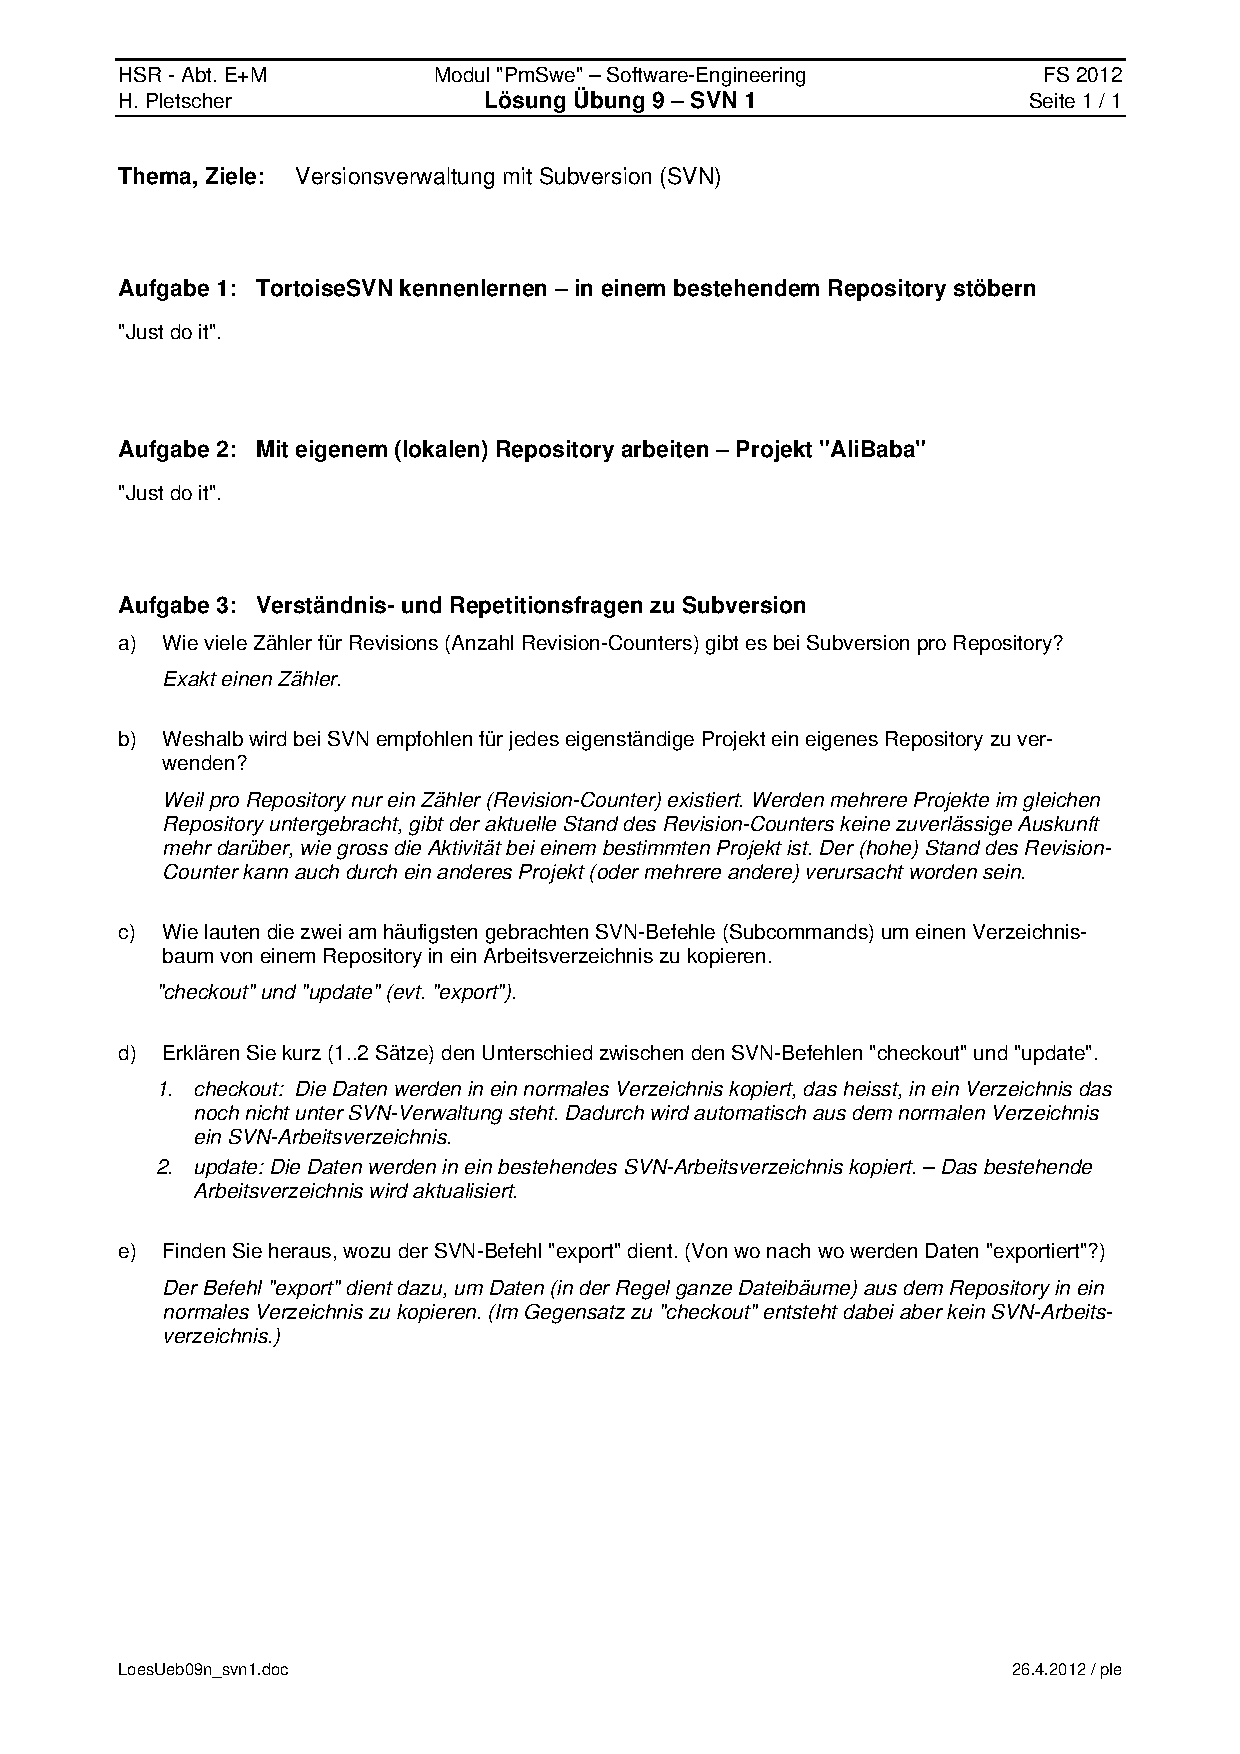
\includepdf[pages=-]{./UebLoesungen/LoesUeb09_svn1/LoesUeb09n_svn1.pdf}

%Uebung 10
\setcounter{section}{10}
\setcounter{subsection}{1}
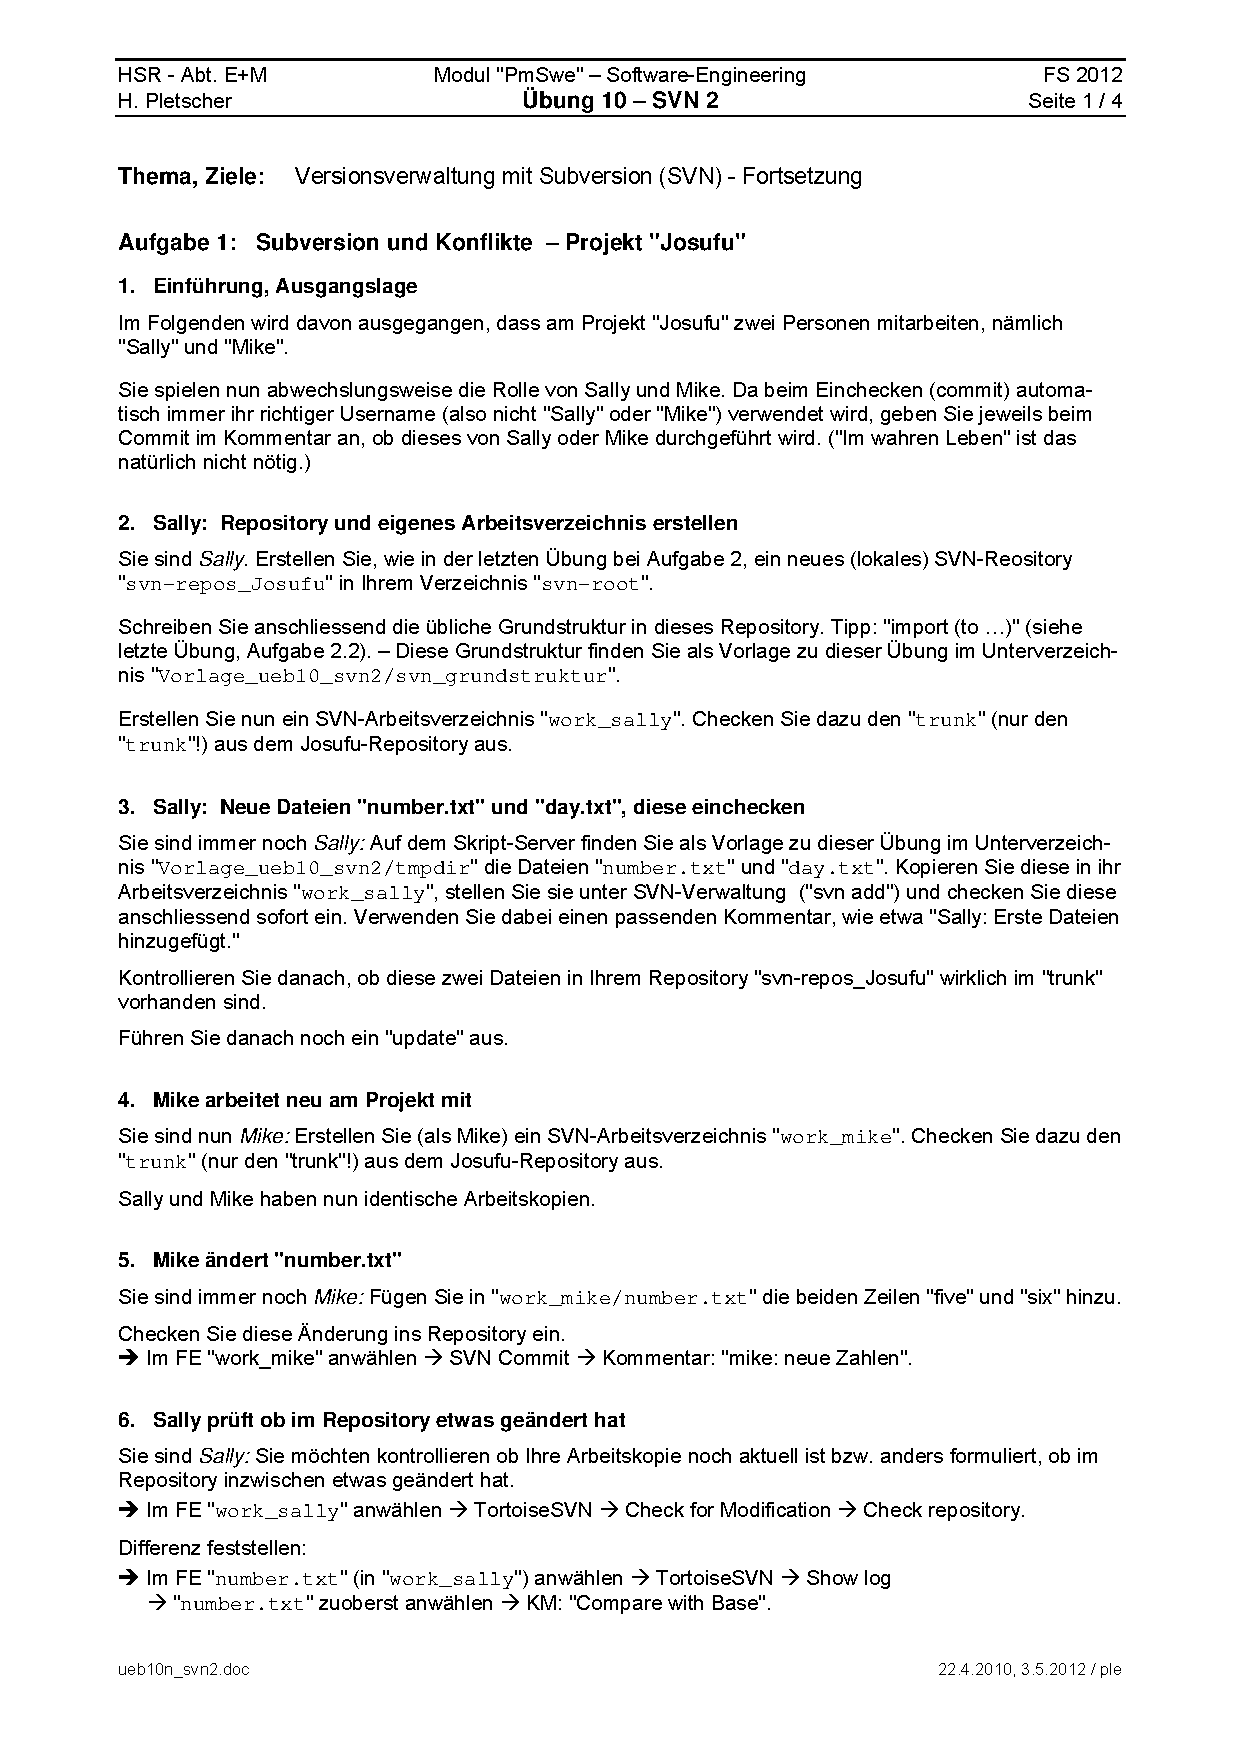
\includepdf[pages=-]{./UebAufgaben/ueb10n_svn2.pdf}

%Uebung 11
\setcounter{section}{11}
\setcounter{subsection}{1}
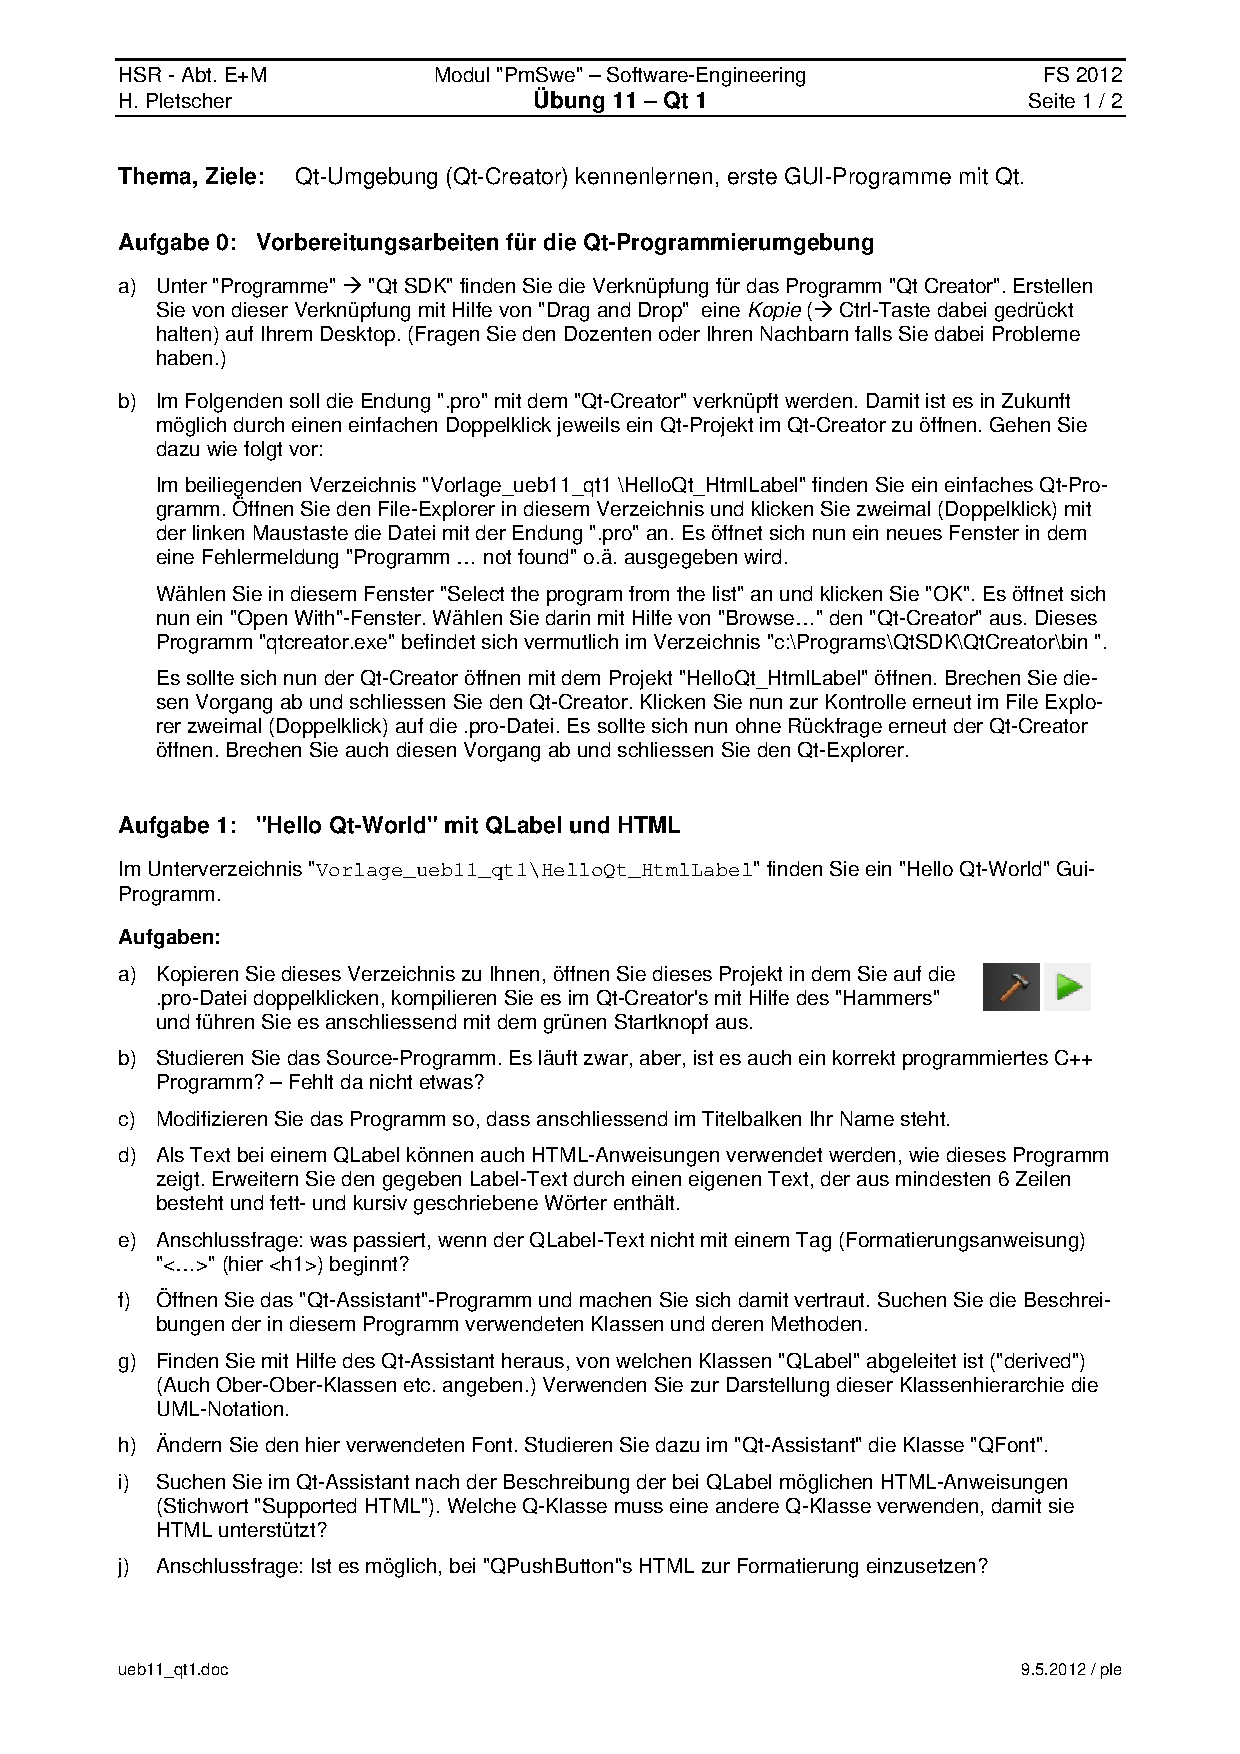
\includepdf[pages=-]{./UebAufgaben/ueb11_qt1.pdf}
\subsection{Lösung Aufgabe 1}
\subsubsection{main.cpp}
\lstinputlisting{./UebLoesungen/LoesUeb11_qt1/lueb11a1_HelloQt_HtmlLabel/main.cpp}
\subsubsection{Qt-Output}
\begin{center}
	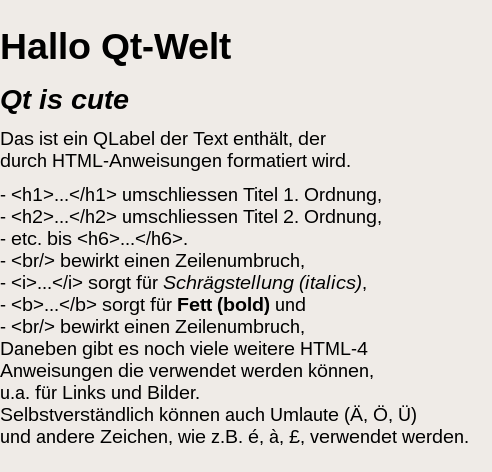
\includegraphics[scale=.5]{./images/u11a1.png}
\end{center}

\subsection{Lösung Aufgabe 2}
\subsubsection{main.cpp}
\lstinputlisting{./UebLoesungen/LoesUeb11_qt1/lueb11a2_HelloQt_PosLabel/main.cpp}
\begin{center}
	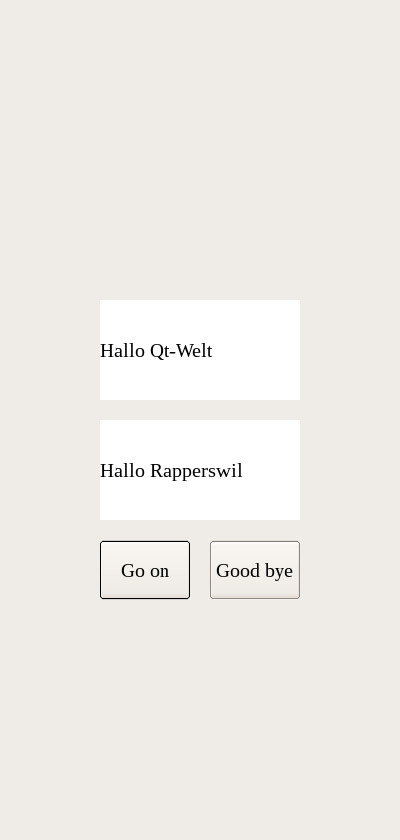
\includegraphics[scale=.5]{./images/u11a2.png}
\end{center}
\subsection{Lösung Aufgabe 3}
\subsubsection{main.cpp}
\lstinputlisting{./UebLoesungen/LoesUeb11_qt1/lueb11a3_HelloQt_Quit/main.cpp}

%Uebung 12
\setcounter{section}{12}
\setcounter{subsection}{1}
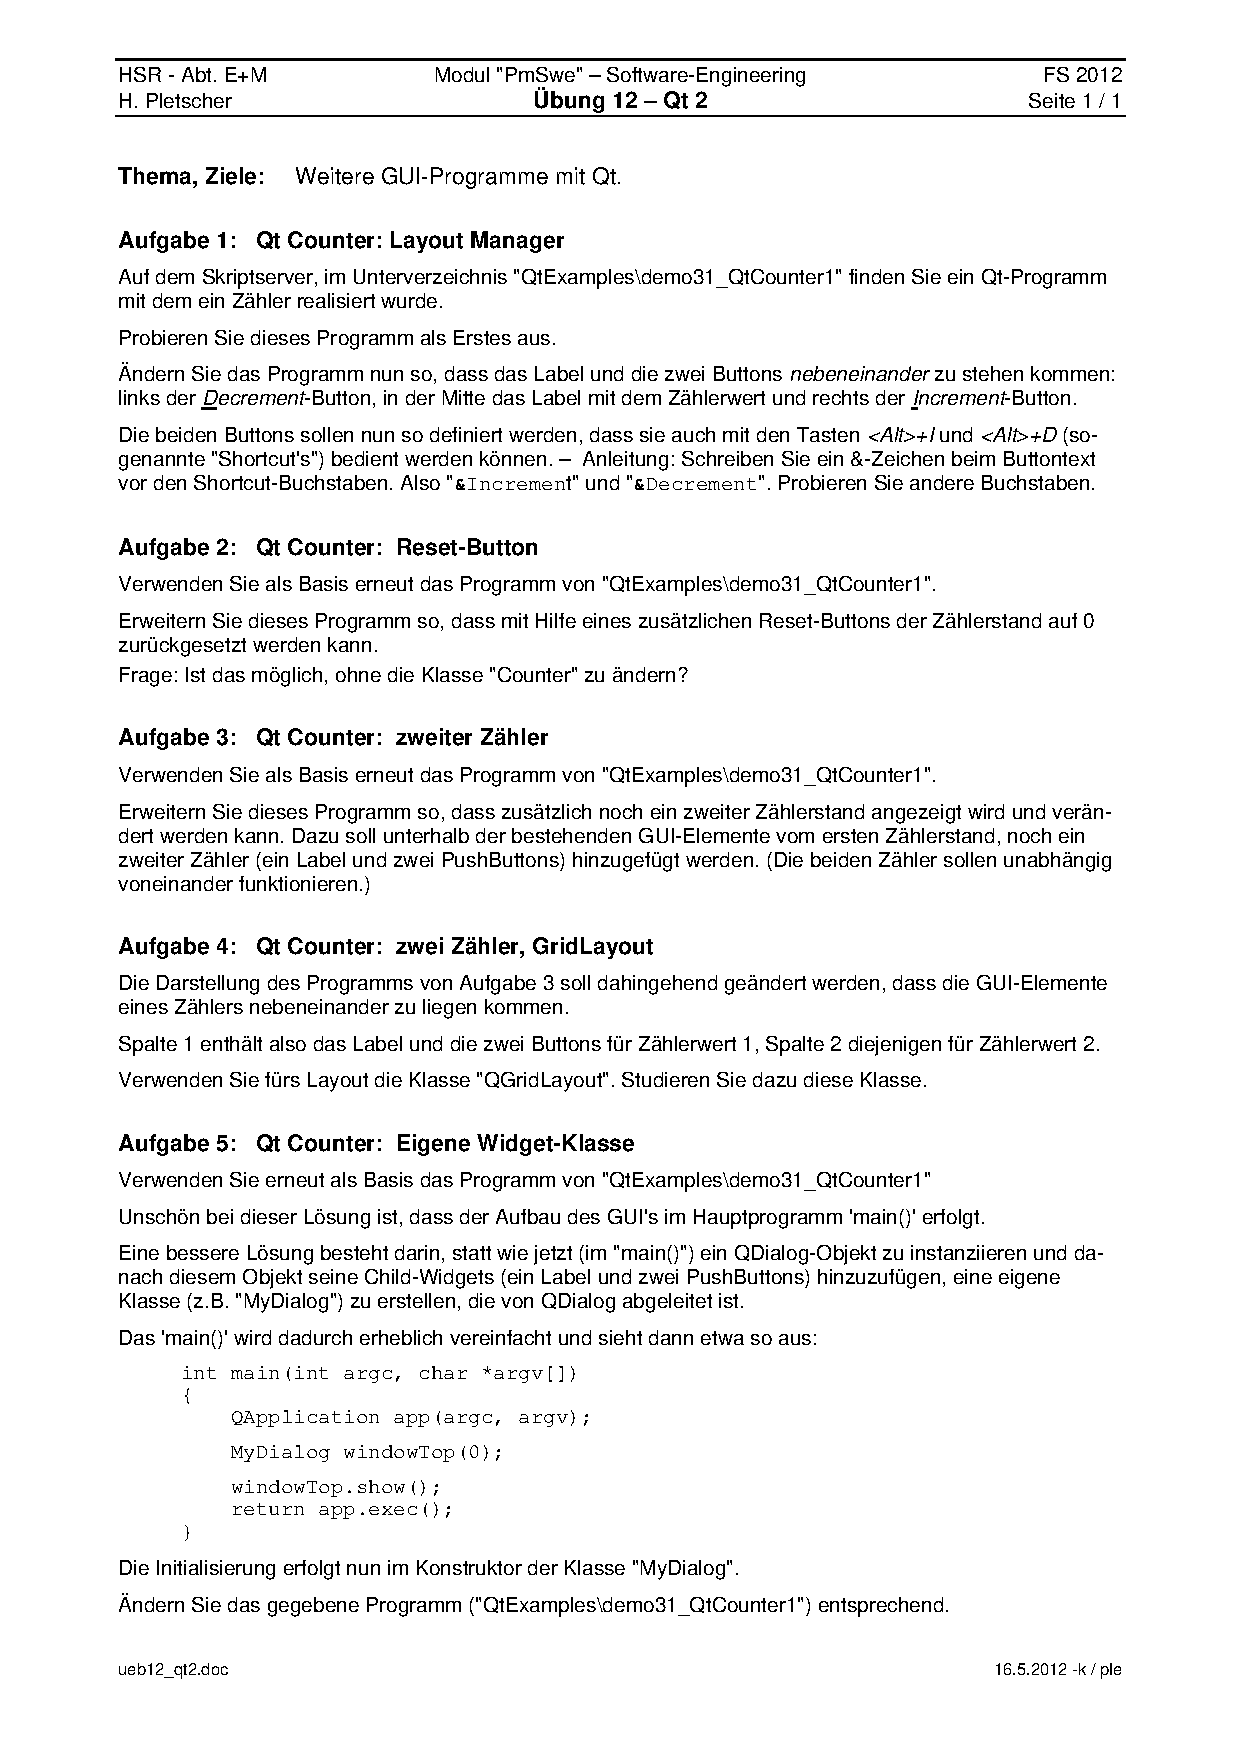
\includepdf[pages=-]{./UebAufgaben/ueb12_qt2.pdf}
\subsection{Lösung}
\subsection{Lösung Aufgabe 1}
\subsubsection{main.cpp}
\lstinputlisting{./UebLoesungen/LoesUeb12_qt2/lueb12a1_CounterLayoutManager/main.cpp}
\subsubsection{counter.cpp}
\lstinputlisting{./UebLoesungen/LoesUeb12_qt2/lueb12a1_CounterLayoutManager/counter.cpp}
\subsubsection{counter.h}
\lstinputlisting{./UebLoesungen/LoesUeb12_qt2/lueb12a1_CounterLayoutManager/counter.h}
\subsubsection{Qt-Output}
\begin{center}
	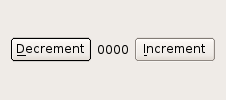
\includegraphics[scale=.5]{./images/u12a1.png}
\end{center}

\subsection{Lösung Aufgabe 2}
\subsubsection{main.cpp}
\lstinputlisting{./UebLoesungen/LoesUeb12_qt2/lueb12a2_CounterResetButton/main.cpp}
\subsubsection{counter.cpp}
\lstinputlisting{./UebLoesungen/LoesUeb12_qt2/lueb12a2_CounterResetButton/counter.cpp}
\subsubsection{counter.h}
\lstinputlisting{./UebLoesungen/LoesUeb12_qt2/lueb12a2_CounterResetButton/counter.h}
\subsubsection{Qt-Output}
\begin{center}
	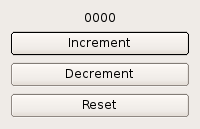
\includegraphics[scale=.5]{./images/u12a2.png}
\end{center}

\subsection{Lösung Aufgabe 3}
\subsubsection{main.cpp}
\lstinputlisting{./UebLoesungen/LoesUeb12_qt2/lueb12a3_CounterZweiZaehler/main.cpp}
\subsubsection{counter.cpp}
\lstinputlisting{./UebLoesungen/LoesUeb12_qt2/lueb12a3_CounterZweiZaehler/counter.cpp}
\subsubsection{counter.h}
\lstinputlisting{./UebLoesungen/LoesUeb12_qt2/lueb12a3_CounterZweiZaehler/counter.h}
\subsubsection{Qt-Output}
\begin{center}
	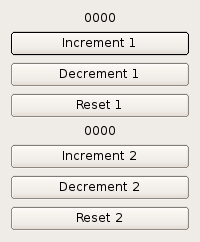
\includegraphics[scale=.5]{./images/u12a3.png}
\end{center}

\subsection{Lösung Aufgabe 4}
\subsubsection{main.cpp}
\lstinputlisting{./UebLoesungen/LoesUeb12_qt2/lueb12a4_CounterGridLayout/main.cpp}
\subsubsection{counter.cpp}
\lstinputlisting{./UebLoesungen/LoesUeb12_qt2/lueb12a4_CounterGridLayout/counter.cpp}
\subsubsection{counter.h}
\lstinputlisting{./UebLoesungen/LoesUeb12_qt2/lueb12a4_CounterGridLayout/counter.h}
\subsubsection{Qt-Output}
\begin{center}
	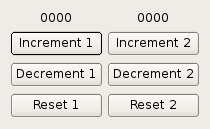
\includegraphics[scale=.5]{./images/u12a4.png}
\end{center}

\subsection{Lösung Aufgabe 5}
\subsubsection{main.cpp}
\lstinputlisting{./UebLoesungen/LoesUeb12_qt2/lueb12a5_CounterWidget/main.cpp}
\subsubsection{Counter.cpp}
\lstinputlisting{./UebLoesungen/LoesUeb12_qt2/lueb12a5_CounterWidget/Counter.cpp}
\subsubsection{Counter.h}
\lstinputlisting{./UebLoesungen/LoesUeb12_qt2/lueb12a5_CounterWidget/Counter.h}
\subsubsection{MyDialog.cpp}
\lstinputlisting{./UebLoesungen/LoesUeb12_qt2/lueb12a5_CounterWidget/MyDialog.cpp}
\subsubsection{MyDialog.h}
\lstinputlisting{./UebLoesungen/LoesUeb12_qt2/lueb12a5_CounterWidget/MyDialog.h}
\subsubsection{Qt-Output}
\begin{center}
	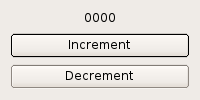
\includegraphics[scale=.5]{./images/u12a5.png}
\end{center}

%Uebung 13
\setcounter{section}{13}
\setcounter{subsection}{1}
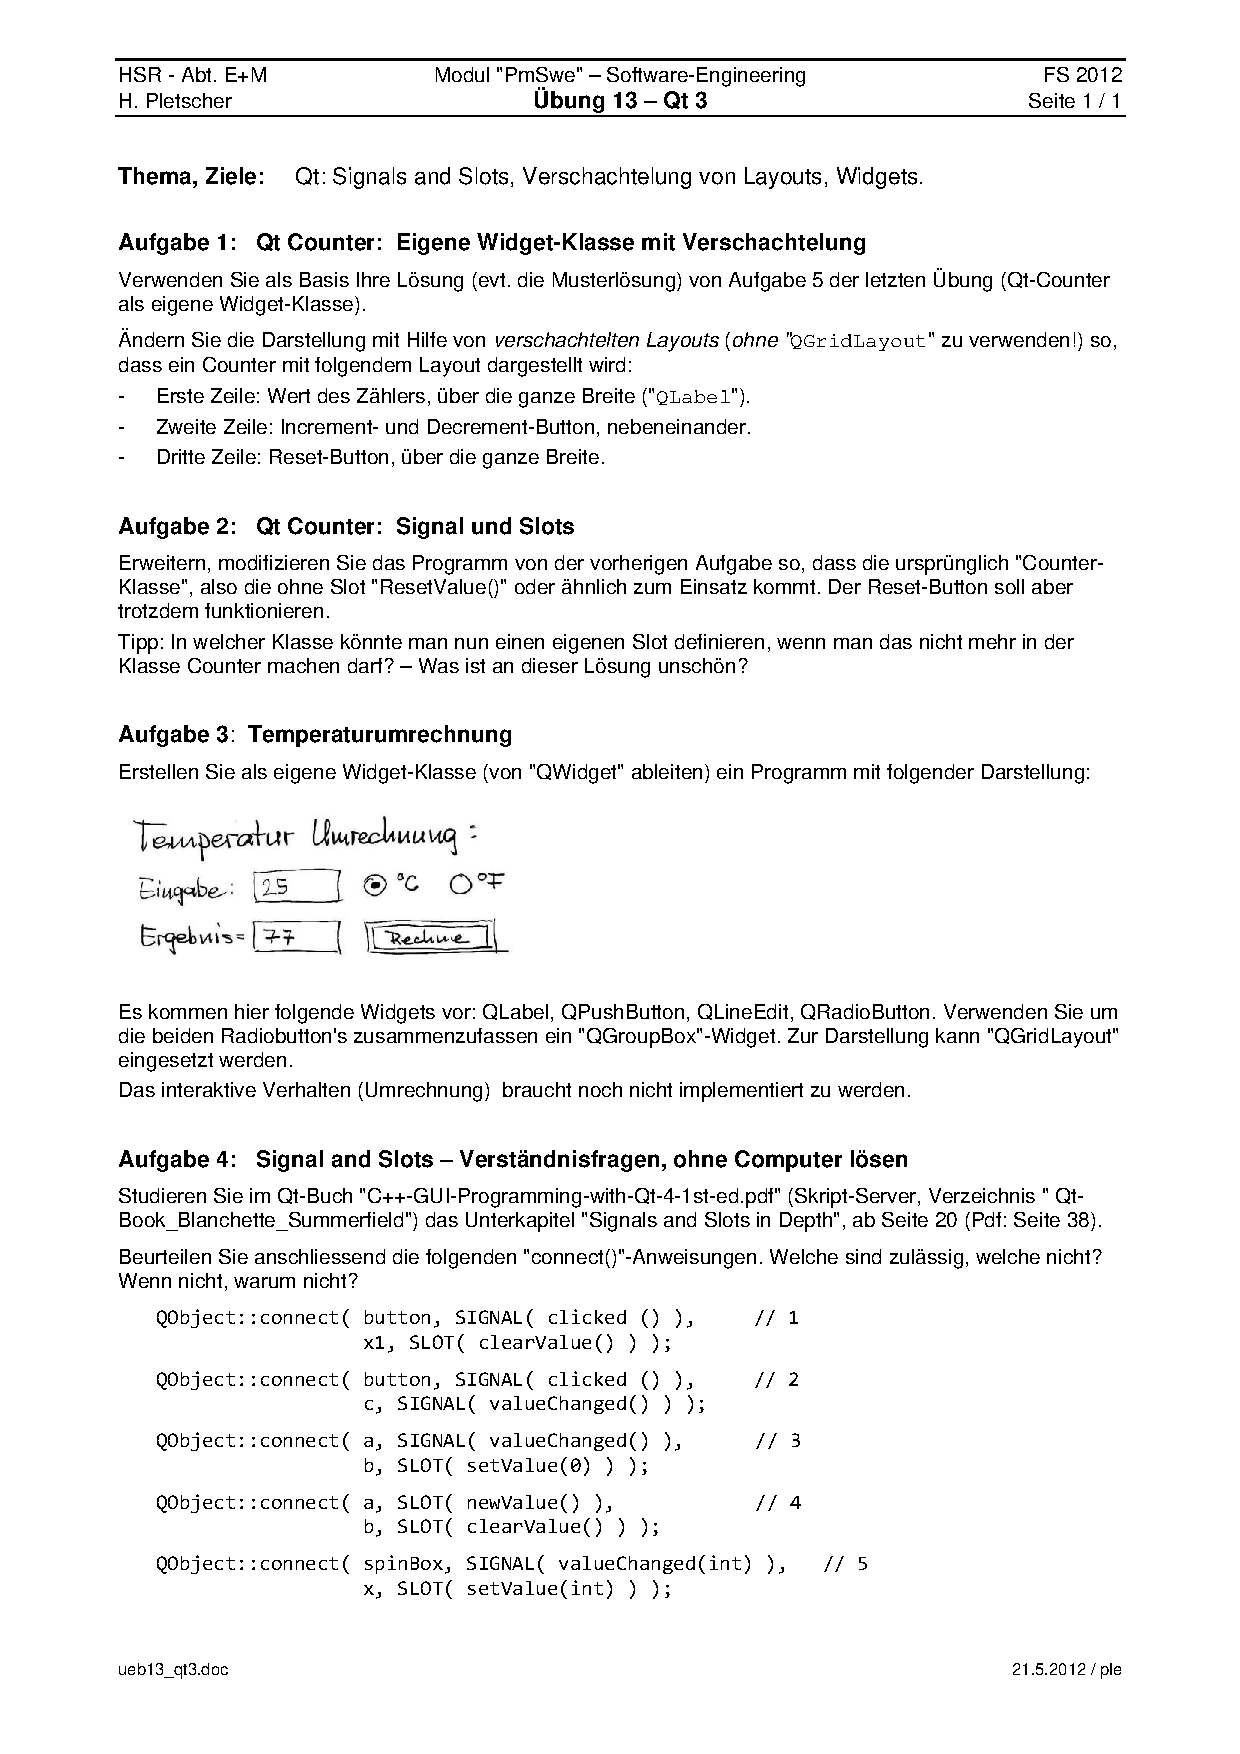
\includepdf[pages=-]{./UebAufgaben/ueb13_qt3.pdf}
\subsection{Lösung Aufgabe 1}
\subsubsection{main.cpp}
\lstinputlisting{./UebLoesungen/LoesUeb13_qt3/lueb13a1_CounterWidgetNested/main.cpp}
\subsubsection{Counter.cpp}
\lstinputlisting{./UebLoesungen/LoesUeb13_qt3/lueb13a1_CounterWidgetNested/Counter.cpp}
\subsubsection{Counter.h}
\lstinputlisting{./UebLoesungen/LoesUeb13_qt3/lueb13a1_CounterWidgetNested/Counter.h}
\subsubsection{MyDialog.cpp}
\lstinputlisting{./UebLoesungen/LoesUeb13_qt3/lueb13a1_CounterWidgetNested/MyDialog.cpp}
\subsubsection{MyDialog.h}
\lstinputlisting{./UebLoesungen/LoesUeb13_qt3/lueb13a1_CounterWidgetNested/MyDialog.h}
\subsubsection{Qt-Output}
\begin{center}
	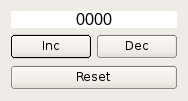
\includegraphics[scale=.5]{./images/u13a1.png}
\end{center}

\subsection{Lösung Aufgabe 2}
\subsubsection{main.cpp}
\lstinputlisting{./UebLoesungen/LoesUeb13_qt3/lueb13a2_CounterOwnSlot/main.cpp}
\subsubsection{Counter.cpp}
\lstinputlisting{./UebLoesungen/LoesUeb13_qt3/lueb13a2_CounterOwnSlot/Counter.cpp}
\subsubsection{Counter.h}
\lstinputlisting{./UebLoesungen/LoesUeb13_qt3/lueb13a2_CounterOwnSlot/Counter.h}
\subsubsection{MyDialog.cpp}
\lstinputlisting{./UebLoesungen/LoesUeb13_qt3/lueb13a2_CounterOwnSlot/MyDialog.cpp}
\subsubsection{MyDialog.h}
\lstinputlisting{./UebLoesungen/LoesUeb13_qt3/lueb13a2_CounterOwnSlot/MyDialog.h}

\subsection{Lösung Aufgabe 3}
\subsubsection{main.cpp}
\lstinputlisting{./UebLoesungen/LoesUeb13_qt3/lueb13a3_TempWidgetView/main.cpp}
\subsubsection{TemperaturWidget.cpp}
\lstinputlisting{./UebLoesungen/LoesUeb13_qt3/lueb13a3_TempWidgetView/TemperaturWidget.cpp}
\subsubsection{TemperaturWidget.h}
\lstinputlisting{./UebLoesungen/LoesUeb13_qt3/lueb13a3_TempWidgetView/TemperaturWidget.h}
\subsubsection{Qt-Output}
\begin{center}
	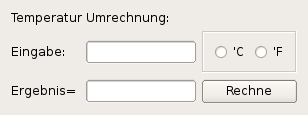
\includegraphics[scale=.5]{./images/u13a3.png}
\end{center}

\subsection{Lösung Aufgabe 4}
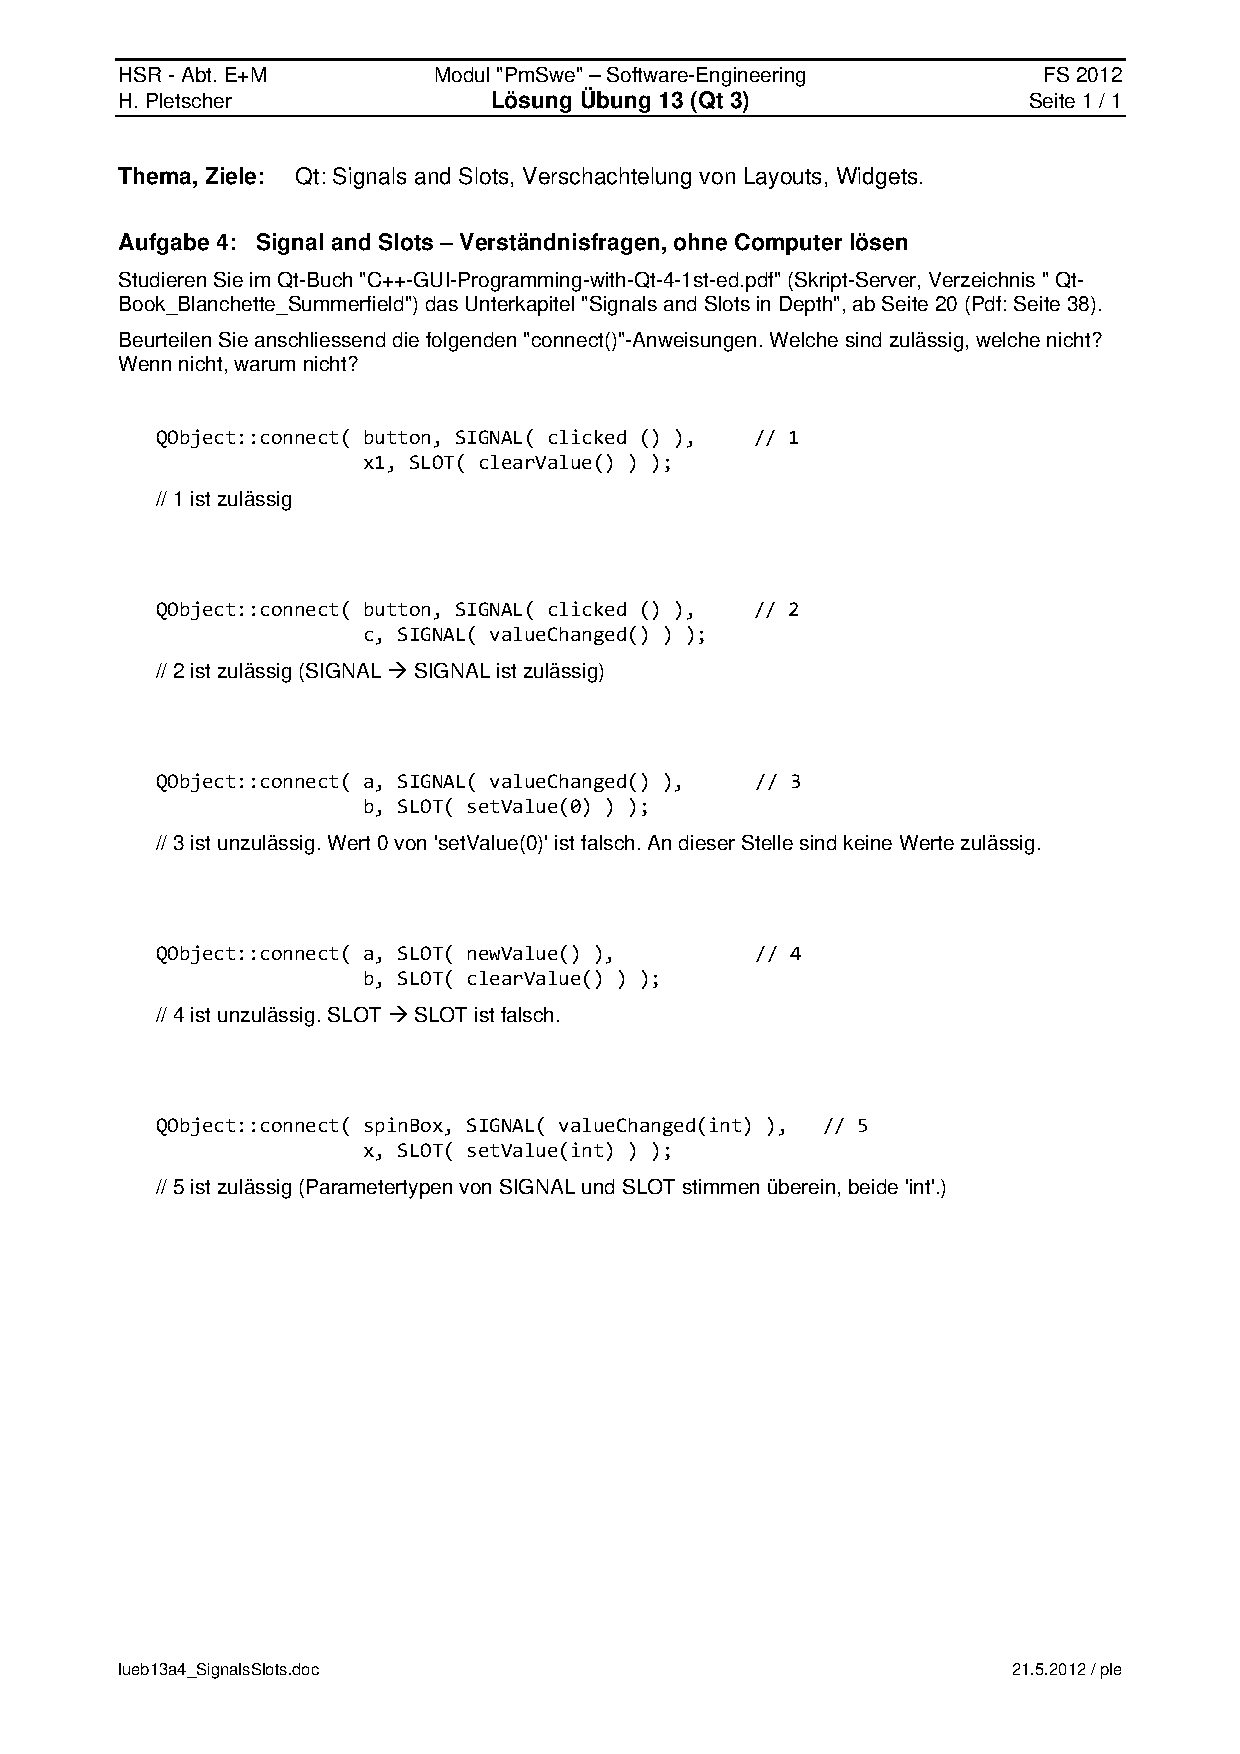
\includepdf[pages=-]{./UebLoesungen/LoesUeb13_qt3/lueb13a4_SignalsSlots.pdf}

%Uebung 14
\setcounter{section}{14}
\setcounter{subsection}{1}
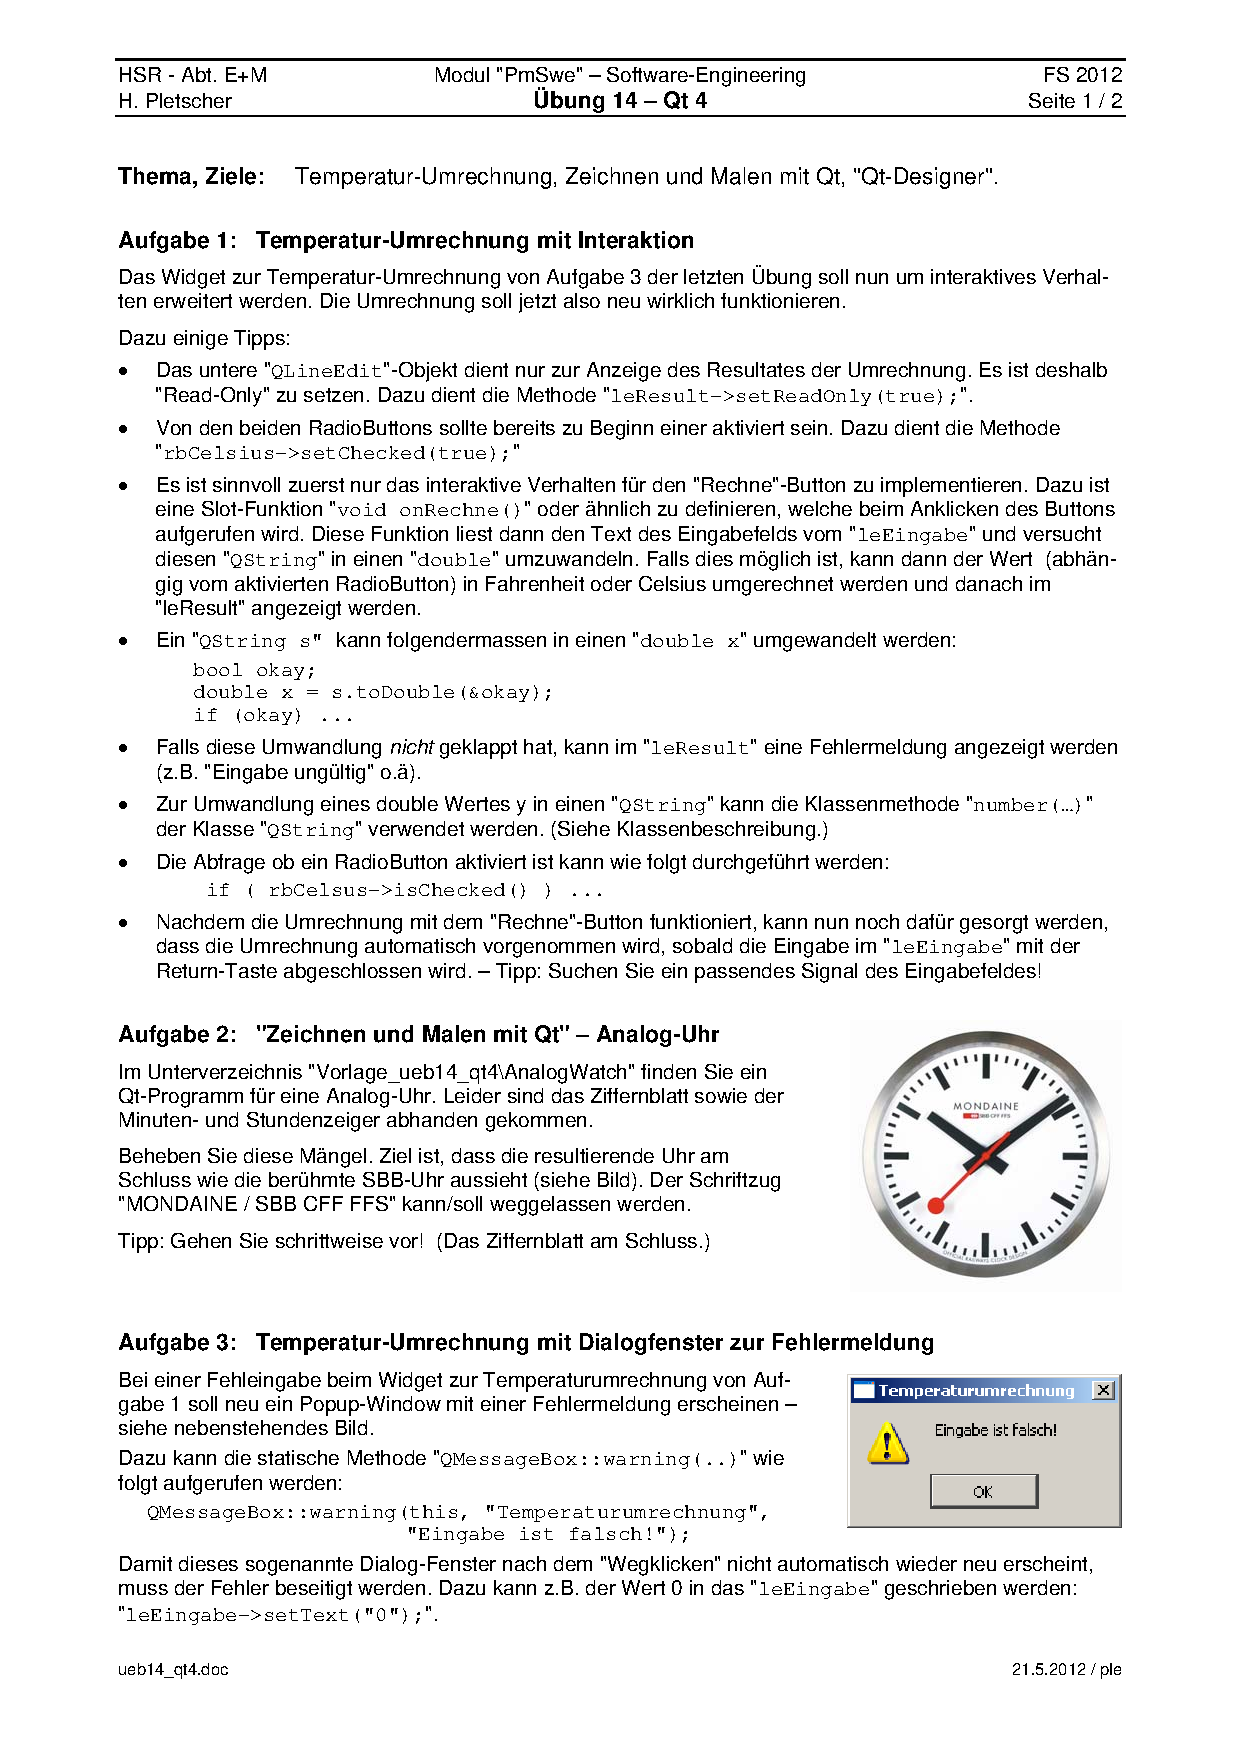
\includepdf[pages=-]{./UebAufgaben/ueb14_qt4.pdf}
\subsection{Lösung Aufgabe 1}
\subsubsection{main.cpp}
\lstinputlisting{./UebLoesungen/LoesUeb14_qt4/lueb14a1_TempWidget/main.cpp}
\subsubsection{TemperaturWidget.cpp}
\lstinputlisting{./UebLoesungen/LoesUeb14_qt4/lueb14a1_TempWidget/TemperaturWidget.cpp}
\subsubsection{TemperaturWidget.h}
\lstinputlisting{./UebLoesungen/LoesUeb14_qt4/lueb14a1_TempWidget/TemperaturWidget.h}
\subsubsection{Qt-Output}
\begin{center}
	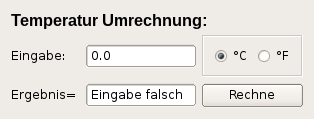
\includegraphics[scale=.5]{./images/u14a1.png}
\end{center}

\subsection{Lösung Aufgabe 2}
\subsubsection{main.cpp}
\lstinputlisting{./UebLoesungen/LoesUeb14_qt4/lueb14a2_AnalogWatch/main.cpp}
\subsubsection{AnalogWatch.cpp}
\lstinputlisting{./UebLoesungen/LoesUeb14_qt4/lueb14a2_AnalogWatch/AnalogWatch.cpp}
\subsubsection{AnalogWatch.h}
\lstinputlisting{./UebLoesungen/LoesUeb14_qt4/lueb14a2_AnalogWatch/AnalogWatch.h}
\subsubsection{Qt-Output}
\begin{center}
	
\includegraphics[scale=.5]{./images/u14a2.png}
\end{center}

\subsection{Lösung Aufgabe 3}
\subsubsection{main.cpp}
\lstinputlisting{./UebLoesungen/LoesUeb14_qt4/lueb14a3_TempWidgetWithDialog/main.cpp}
\subsubsection{TemperaturWidget.cpp}
\lstinputlisting{./UebLoesungen/LoesUeb14_qt4/lueb14a3_TempWidgetWithDialog/TemperaturWidget.cpp}
\subsubsection{TemperaturWidget.h}
\lstinputlisting{./UebLoesungen/LoesUeb14_qt4/lueb14a3_TempWidgetWithDialog/TemperaturWidget.h}



\end{document}
